\documentclass{article}
\usepackage{graphicx}
\usepackage{hyperref}
\usepackage{amsthm}
\usepackage{amsmath}
\usepackage{amssymb}
\usepackage{listings}
\usepackage{algorithm}
\usepackage[noend]{algpseudocode}

\lstset{basicstyle=\ttfamily}
\newcommand{\code}{\lstinline}

\newtheorem{definition}{Definition}

\title{\small{\textit{Notes on}}\\ \huge{\textit{Foundations of \\ Artificial Intelligence}}}
\author{Fabio Vokrri}
\date{2024-2025}

\begin{document}

\maketitle
\newpage
\tableofcontents

\clearpage
\section{Introduction}
There isn't a single definition of Artificial Intelligence: some define intelligence in terms of fidelity to human performance, while others prefer a formal definition of intelligence called \textbf{rationality}. Some consider intelligence to be a property of reasoning and thought process, while others focus on intelligent behavior.  

From these two characterizations (human v. rational/ thought v. behavior) there are four possible combinations that cross several scientific disciplines.

\subsection{Acting Humanly - Turing Test Approach}
Alan Turing proposed the Turing test, a mental experiment to answer the question whether or not a computer can reach human-like performance. The test is passed if a human interrogator, after posing some written questions, cannot tell if the written responses came from a person or a computer.

To pass the test, the computer would need the following capabilities:
\begin{itemize}
    \item Natural language;
    \item Knowledge representation;
    \item Automated reasoning;
    \item Machine learning.
\end{itemize}

\subsection{Thinking Humanly - Cognitive Modeling Approach}
In order to say that a program thinks like a human, we must know how humans think. We can learn about human thoughts via an approach called \textbf{cognitive modeling} in three main ways:
\begin{enumerate}
    \item Introspection: trying to capture our own thoughts;
    \item Psychological experiments: observing human behavior;
    \item Brain imaging: observing the brain in action.
\end{enumerate}

Once we have a precise theory of the mind, it can be said that if a program's input-output behavior matches a corresponding human behavior, that is evidence that some of the program's mechanisms could also be present in a human. 

\subsection{Thinking Rationally - "Laws of thought" Approach}
This approach is based on the laws of thought, which provide a way to yield correct conclusions given the right premises. The field that studies this laws is called \textbf{logic} and requires the knowledge of the world that is certain,  a condition rarely met in reality. The theory of probability fills the gap, allowing rigorous reasoning with uncertain information.

\subsection{Acting Rationally - Rational Agent Approach}
An agent is something that autonomously acts, perceives the environment, persists over a prolonged period of time, adapts to the changes and pursues a goal. A rational agent is one that acts to achieve the best outcome.
This approach of AI has prevailed throughout the field's history because it's more general and amenable to scientific approach than others. AI has focused on the study of agents that do the right thing.

\clearpage
\section{Intelligent Agents}
An agent is anything that can be viewed as perceiving its environment through sensors and acting through actuators: it could be a robot or a software program. The environment is a part of the universe whose state we are interested in when designing the agent, that is what the agent sees and what is effected by the agent's actions.

We use the term \textbf{percept} to refer to the content that the agent's sensors are perceiving. A \textbf{percept sequence} is the complete history of everything the agent has perceived.

An agent's action at any given time depends on its built-in knowledge and on the entire percept sequence observed to date, but not in anything it hasn't perceived. Mathematically speaking, it can be said that an agent's behavior is described by the agent function, that maps any given percept sequence to an action the agent can perform.

\subsection{Good Behavior and Rationality}
In order to define an agent rational, it must choose the "right" action, which is described by the notion of \textbf{consequentialism}: we evaluate an agent's behavior based on its consequences. When we introduce an agent to the environment, it produces a sequence of actions according to the percepts it receives. These actions cause the environment to go through a sequence of states and, if this sequence is desirable, then the agent has performed well. This notation of desirability is captured by a \textbf{performance measure}, which is the criterion for evaluating the performance of an agent and it is initially prompted to the agent by its designer.

The action that the agent must choose in order to be called rational depends on four main thing:
\begin{enumerate}
    \item Performance measure, which defines the criteria for success;
    \item Agent's prior knowledge of the environment;
    \item Actions that the agent can perform;
    \item Agent's percept sequence up to date.
\end{enumerate}

We can finally give a definition of a rational agent:
\begin{definition}[Rational Agent]
For each possible percept sequence, a rational agent should select an action that is expected to maximize its performance measure, given the evidence provided by the percept sequence and whatever built-in knowledge the agent has.
\end{definition}

Formally, at time $t$ an agent program outputs an action $a(t)$, given the current perception $p(t)$ and all previous perceptions $p(0), p(1), ..., p(t-1)$).

\subsection{Nature of Environments}
Before approaching the design of a rational agent, we must think about \textbf{task environments}, that are the problems that the agent is trying to solve. The nature of the task environments directly affects the appropriate design for the agent. The range of tasks environments that might arise in AI is vast, but can be categorized as follows:
\begin{description}
    \item[Fully v. Partially Observable] If an agent's sensors give it access to the complete state of the environment at each point in time, then we say that the task environment is fully observable.
    A task environment is effectively fully observable if the sensors detect all aspects that are relevant to the choice of action. 
    Fully observable environments are convenient because the agent doesn't need to maintain any interval state to keep track of the world.
    An environment could be partially observable because of noisy and inaccurate sensors or because part of the state are missing from the sensor data. If the agent has no sensors, the environment is unobservable.

    \item[Single v. Multi Agent] Whether or not there are more than one agent operating in the task environment. But not all actors in an environment can be considered agents. A key factor to identify an agent is whether an entity behavior is best described as maximizing a performance measure whose value depends on another agent's behavior. 
    If an entity us trying to maximize its performance measure by minimizing another agent's performance measure, then we can call the environment \textbf{competitive}, otherwise is called \textbf{cooperative}.

    \item[Deterministic v. Non-deterministic] If the next state of the environment is completely determined by the current state and the action executed by the agent (or agents), then we can sat that the environment is deterministic, otherwise is non-deterministic.
    If the environment is partially observable, it could appear to be non-deterministic. Furthermore, we say that the model is \textbf{stochastic} if it explicitly deals with quantified probabilities and it is non-deterministic if the probabilities are listed, but not quantified.

    \item[Episodic v. Sequential] In an episodic task environment, the agent's experience is divided into atomic episodes, in which the agent receives a single percept and performs a single action. Furthermore, the next episode does not depend on the actions taken in previous episodes. In sequential environments, on the other hand, the current decision can effect future decisions.

    \item[Static v. Dynamic] If the environment can change while an agent is deliberating, the environment is said to be dynamic for that agent, otherwise is static. Static environments are easy to deal with because the agent needs not to keep looking at the world while deciding on an action to take. If the environment does not change with the passage of time, but the agent's performance score does, the environment is said to be \textbf{semi-dynamic}.

    \item[Discrete v. Continuous] This distinction applies to the state of the environment, to the way time is handled, and the percepts and actions of the agent.

    \item[Known v. Unknown] This distinction does not apply to the environment, but to the agent itself, more precisely to the agent's state of knowledge about the lows of physics of the environment. In a known environment, the outcome of any possible action is given, otherwise the agent must learn how it works in order to make good decisions.
\end{description}

\noindent
Here it is a table of the most famous AI problems and its environments:
\begin{figure}[h]
    \centering
    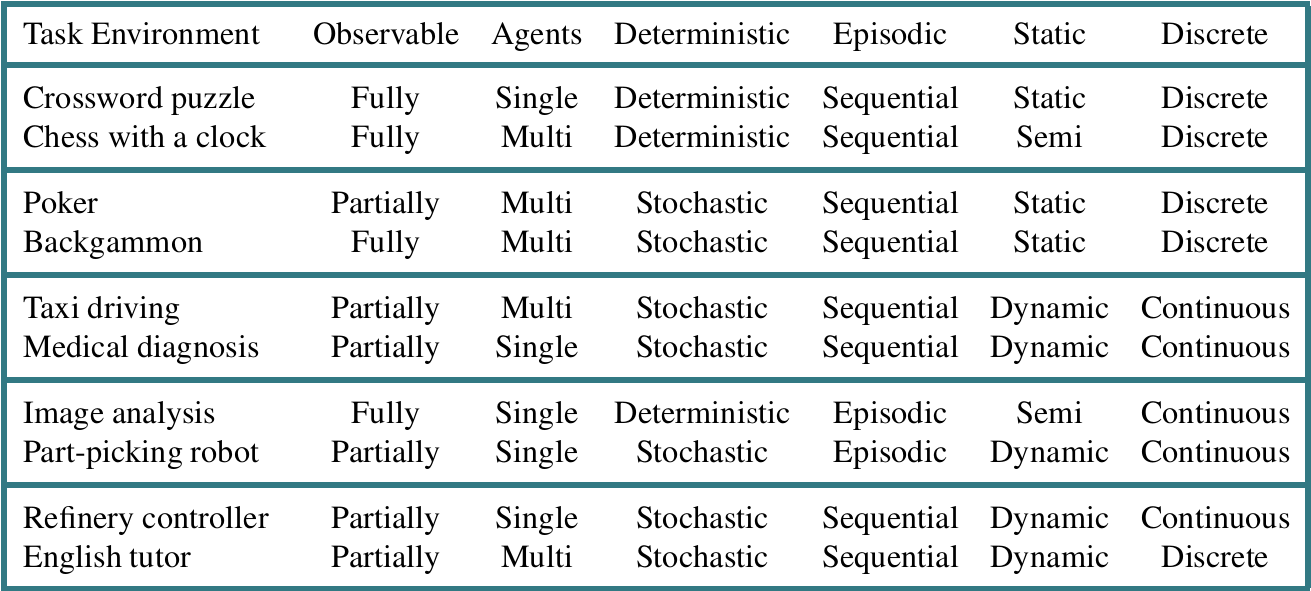
\includegraphics[width=0.85\linewidth]{images/Task Environments.png}
    \caption{Examples of task environments and their characteristics}
    \label{fig:task_nvironments}
\end{figure}

\subsection{The Structure of Agents}
The job of an AI is to design an agent's program that produces rational behavior. There are four categories of agent programs:
\begin{enumerate}
    \item Simple reflex agent.
    \item Model-based agent.
    \item Goal-based agent.
    \item Utility-based agent.
\end{enumerate}

Each type of agent combines some components in particular ways to generate actions.

\subsubsection{Simple Reflex Agents}
The simplest kind of agent is the Simple Reflex Agent, that select actions on the basis of the current percept, ignoring all the percept history. The actions taken by this kind of agent are given by some condition-action rules, which are simple \code{if-then-else} statements that return a single action based on the current status of the environment.

\begin{figure}[h]
    \centering
    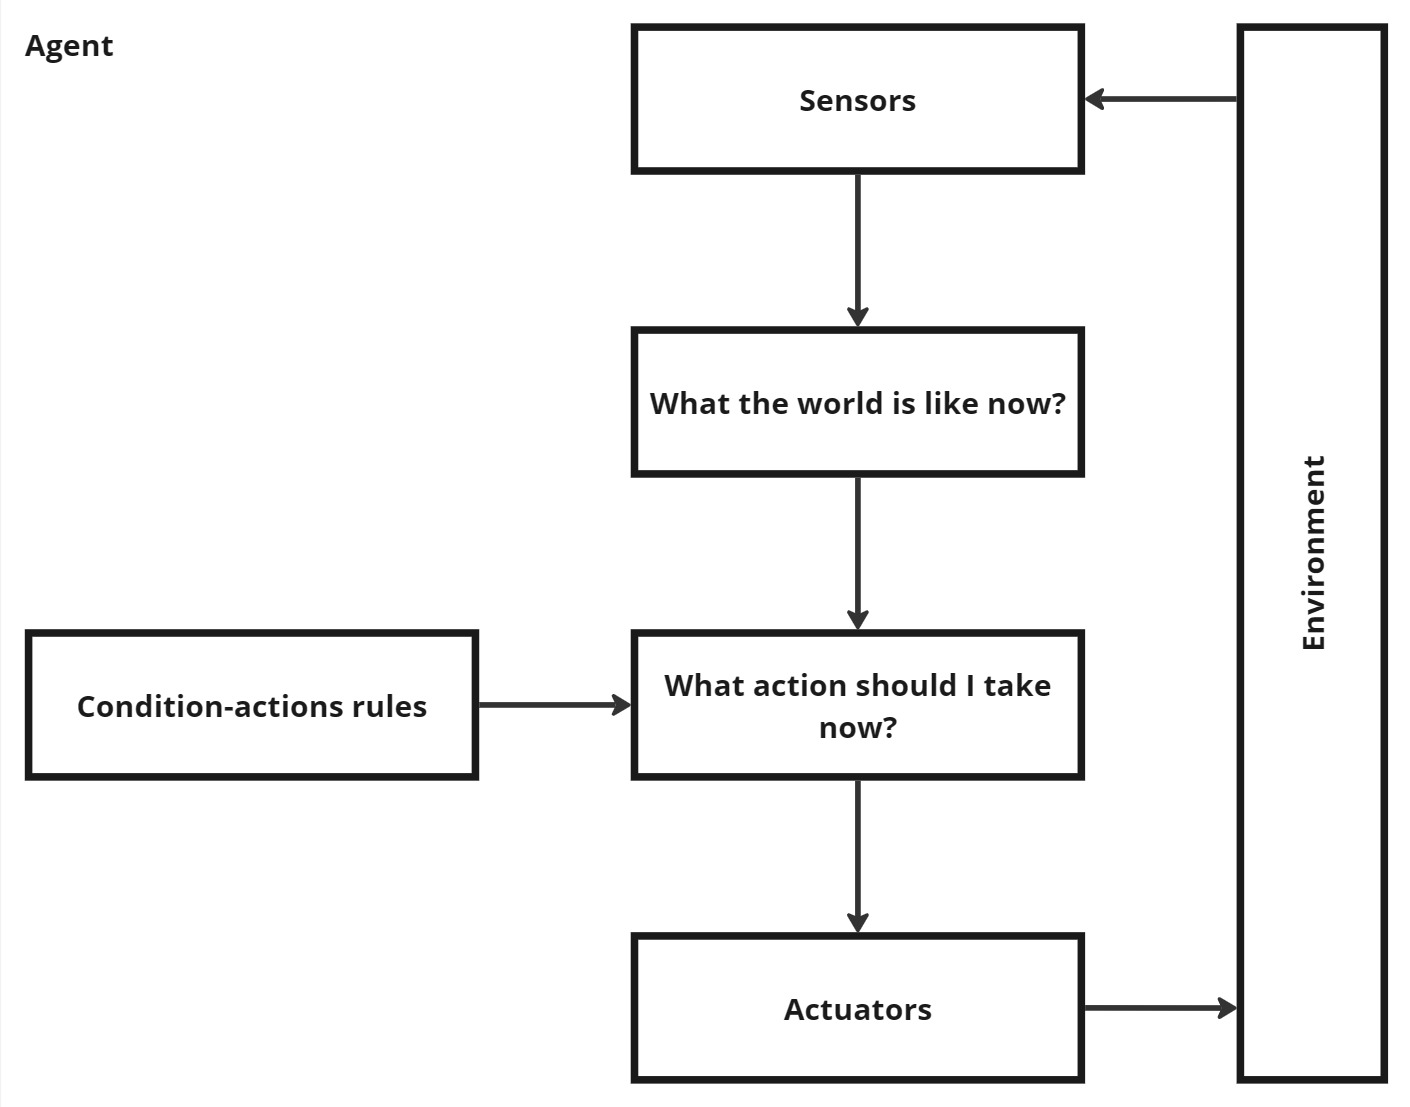
\includegraphics[width=0.5\linewidth]{images/Simple Reflex Agent.jpg}
    \caption{Simple Reflex Agent}
    \label{fig:simple_reflex_agent}
\end{figure}

Simple reflex agents are incredibly simple, but they have really limited intelligence. The agent will work only if the environment is fully observable and even a little bit of unobservability can cause the agent to fail. Additionally, this kind of agents can fall into infinite loops of actions that are useless. To avoid this situation, some agents randomize actions, outperforming a deterministic version of the same agent. 

\vspace{5mm}
\begin{algorithmic}
\Function{Simple-Reflex-Agent}{$percept$}{ \textbf{returns} an action}
    \State \textbf{persistent}: $rules$, a set of condition-action rules
    \State
    \State $state \gets$ \Call{Interpret-Input}{$percept$}
    \State $rule\gets$ \Call{Rule-Match}{$state$, $rules$}
    \State $action\gets rule.$\Call{Action}{}
    \State \Return $action$
\EndFunction
\end{algorithmic}
\vspace{5mm}

\subsubsection{Model-Based Reflex Agents}
The most effective way to handle partial observability is for the agent to keep track of the part of the world it cannot see at the moment. The agent should maintain some sort of internal state that depends on the percept history and therefore reflects some of the under-observed aspects of the environment.

\clearpage
\begin{figure}[h]
    \centering
    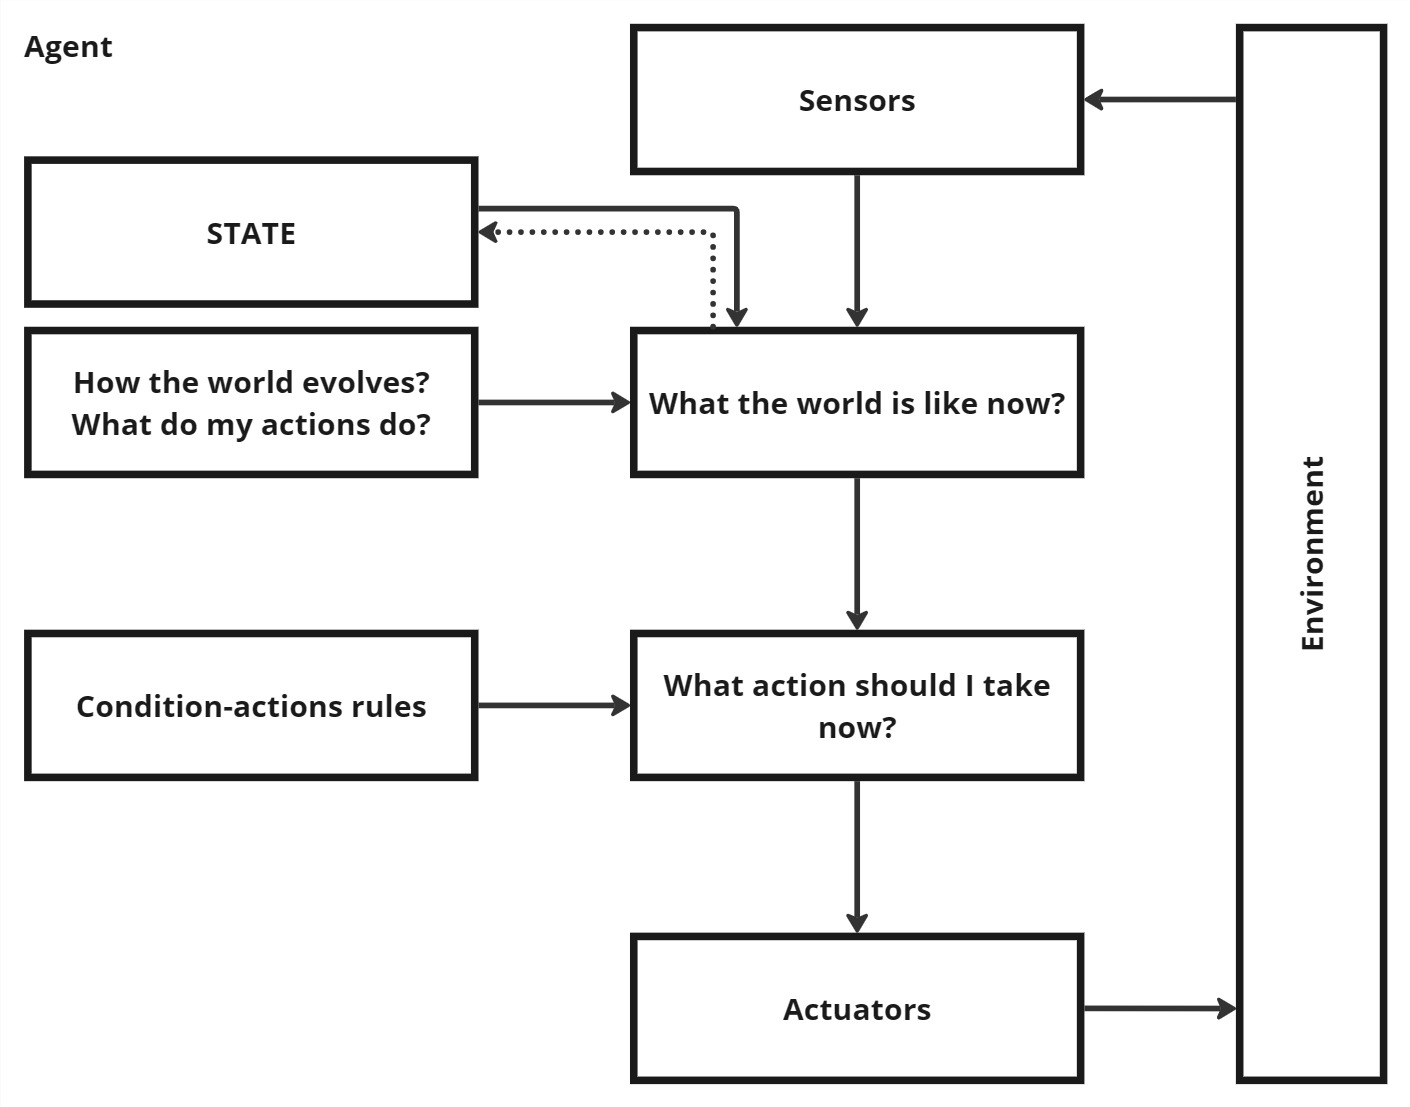
\includegraphics[width=0.5\linewidth]{images/Model Based Reflex Agent.jpg}
    \caption{Model Based Reflex Agent}
    \label{fig:model_based_reflex_agent}
\end{figure}

To update its internal state information, the agent's program must encode two types of knowledge
\begin{enumerate}
    \item Information about how the world changes over time, which can be divided in two parts:
    \begin{itemize}
        \item The effects of the agent's actions;
        \item How the world evolves independently of the agent.
    \end{itemize}
    This knowledge about how the world evolves is called a \textbf{transition model};
    \item Information about how the state of the world is reflected in the agent's percepts. This kind of knowledge is called \textbf{sensor model}.
\end{enumerate}
Together, the transition model and the sensor model allow the agent to keep track of the state of the world. An agent that uses such models is called a model-based agent.

A basic algorithm to model a model-based reflex agent is the following:
\begin{figure}[h]
    \centering
    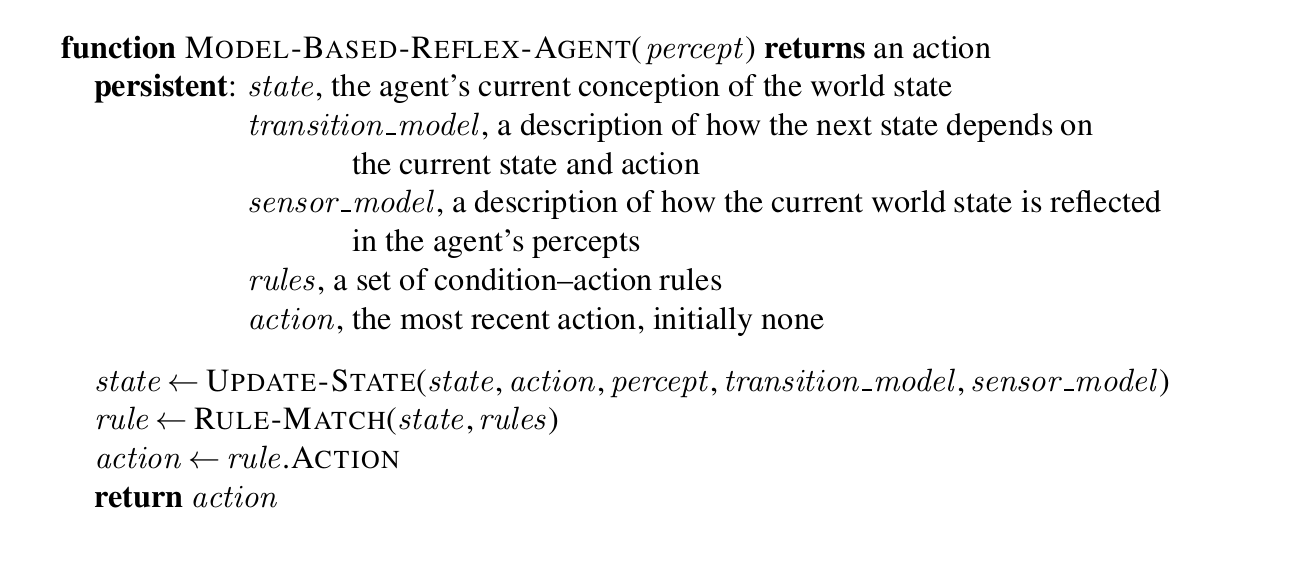
\includegraphics[width=\linewidth]{algorithms/Model Based Reflex Agent.png}
    \label{fig:model_based_reflex_agent_algorithm}
\end{figure}

\subsubsection{Goal-Based Agents}
Knowing something about the current state of the environment is not always enough to decide what to do. As well as the current state description, the agent needs some sort of \textbf{goal}, which are pieces of information that describe desirable situations. The decision making part of this type of agent is different from the condition-action rules found in the model based reflex agents, in that involves some considerations of the future.

\begin{figure}[h]
    \centering
    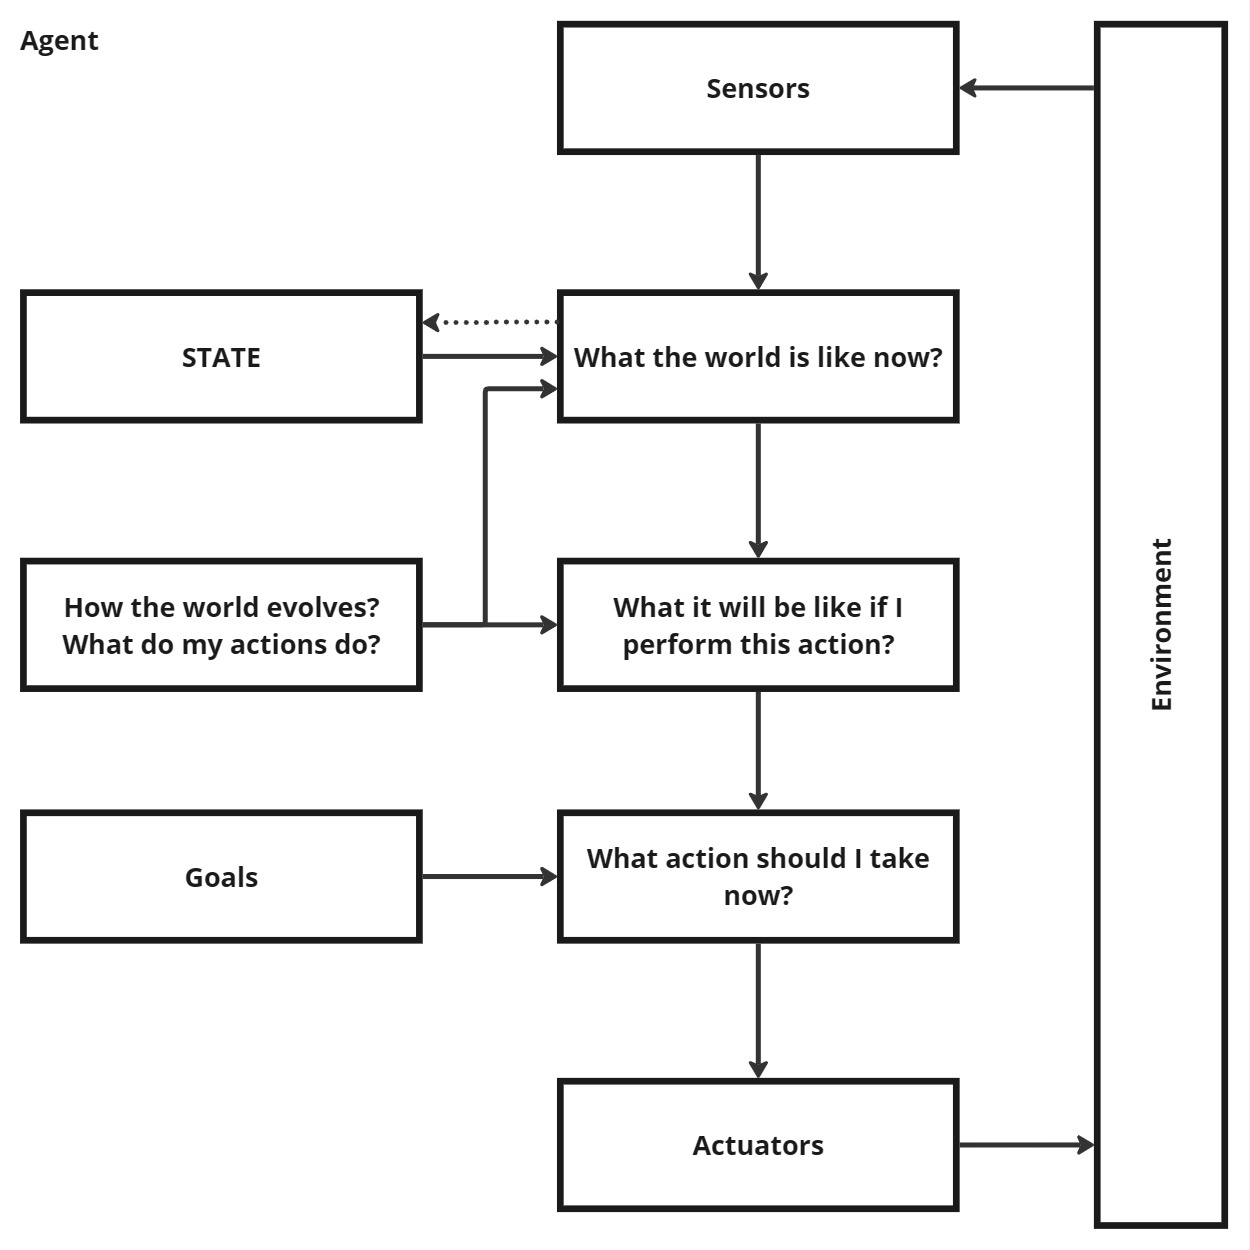
\includegraphics[width=0.5\linewidth]{images/Goal Based Agent.jpg}
    \caption{Goal Based Agent}
    \label{fig:goal_based_agent}
\end{figure}

Agents of this kind may appear less efficient than the ones analyzed up to now, but in reality they are more flexible because the knowledge that supports its decisions is represented explicitly and can be modified, simply by specifying the new goal.

\subsubsection{Utility-Based Agents}
Goals alone are not enough to produce high quality behavior in most environments, because they only provide a crude distinction between "happy" and "unhappy" states. A so called \textbf{utility function} provides a way in which the likelihood of success can be weighted against the importance of the goals, and can help identify the best trade-off between conflicting goals.

An agent's utility function is an internalization of the performance measure. Provided that the internal utility function and the external performance measure are in agreement, an agent that chooses actions to maximize its utility function will be rational according to the external performance measure. 

\clearpage
\begin{figure}[h]
    \centering
    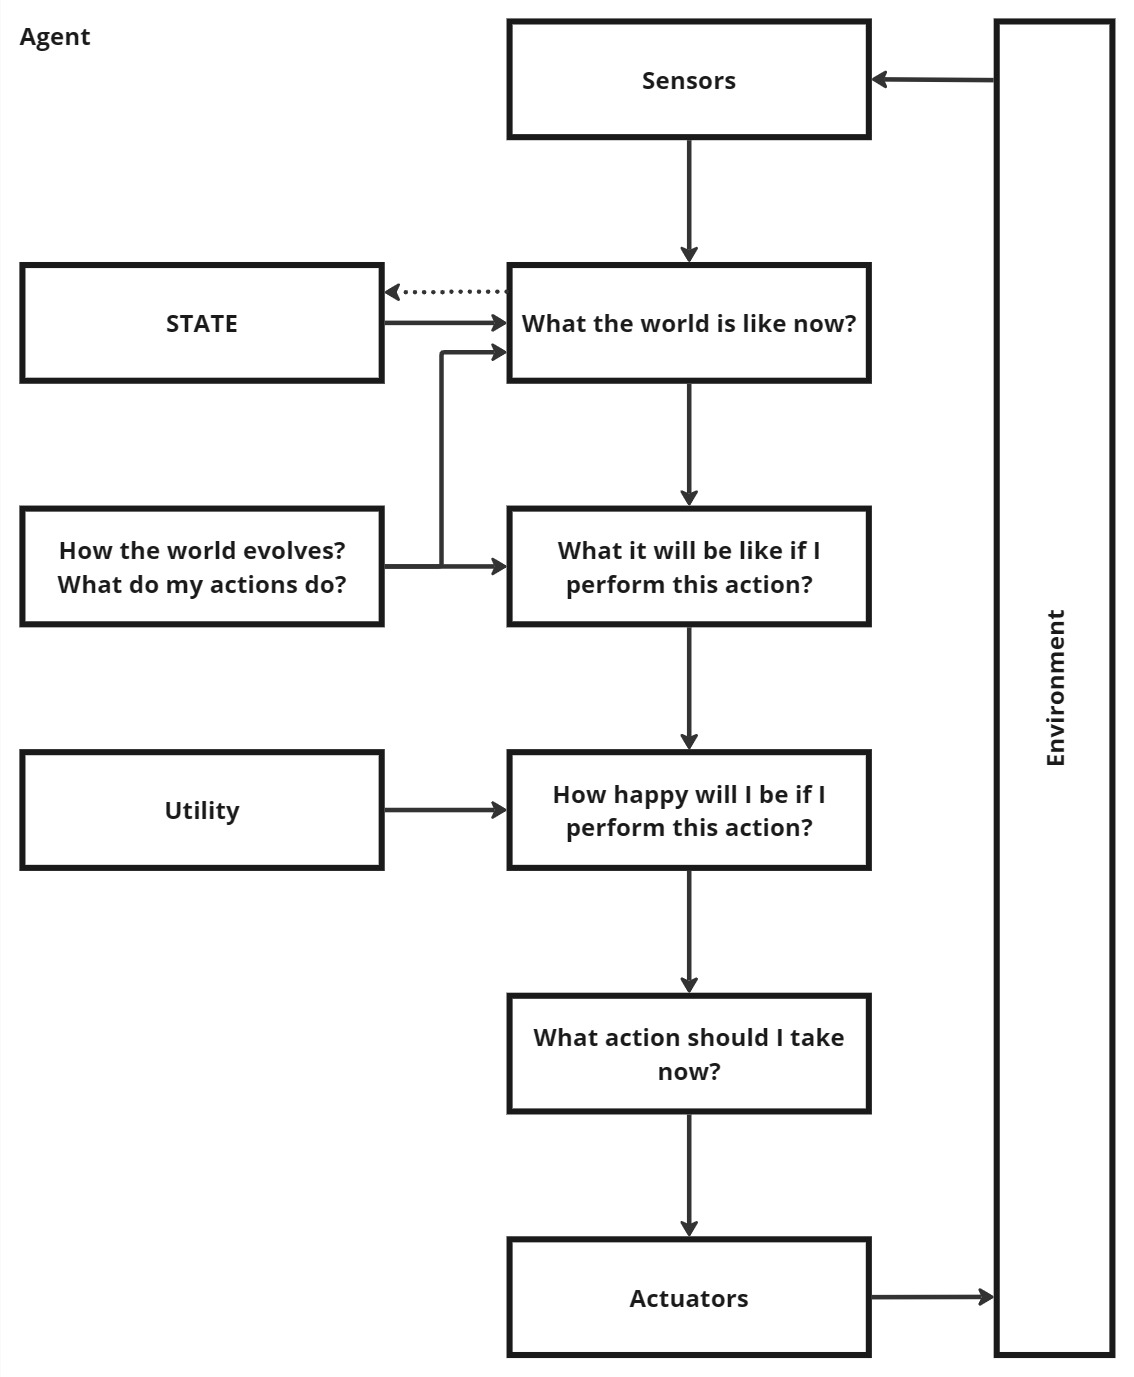
\includegraphics[width=0.5\linewidth]{images/Utility Based Agent.jpg}
    \caption{Utility Based Agent}
    \label{fig:utility_based_agent}
\end{figure}

There are two cases where goals are inadequate, but utility-based agents can still make rational decisions:
\begin{enumerate}
    \item Where there are conflicting goals but only some of them can be achieved: in this case the utility function specifies the right trade-off between the two goals.
    \item Where there are several goals that the agent can aim for, none of which can be achieved with certainty: in this case the utility function provides a way in which the likelihood of success can be weighted against the importance of the goal.
\end{enumerate}

\subsubsection{Learning Agents}
Any type of agent, such as model-based, goal-based or utility-based, can be built as a learning agent to improve their performance. Learning allows the agent to operate in a initially unknown environment and to become more competent than its initial knowledge alone might allow. It can be divided in four conceptual components:
\begin{enumerate}
    \item \textbf{Learning element}: responsible for making improvements.
    \item \textbf{Performance element}: analyzes the sensor input data and selects external actions. It's what we considered as the entire agent in the previous chapter.
    \item \textbf{Critic}: provides feedback on the actions taken by the agent and determines how the performance element should be modified to improve performance. In other words, it tells the learning element how well the agent is doing with respect to a fixed performance standard. 
    \item \textbf{Problem generator}: suggests exploratory actions that lead to new and informative experiences. It is responsible for suggesting suboptimal actions in the short term, in order to discover much better actions for the long term. The problem generator component might identify certain parts of the model that are in need of improvement and suggest experiments.
\end{enumerate}

\begin{figure}[h]
    \centering
    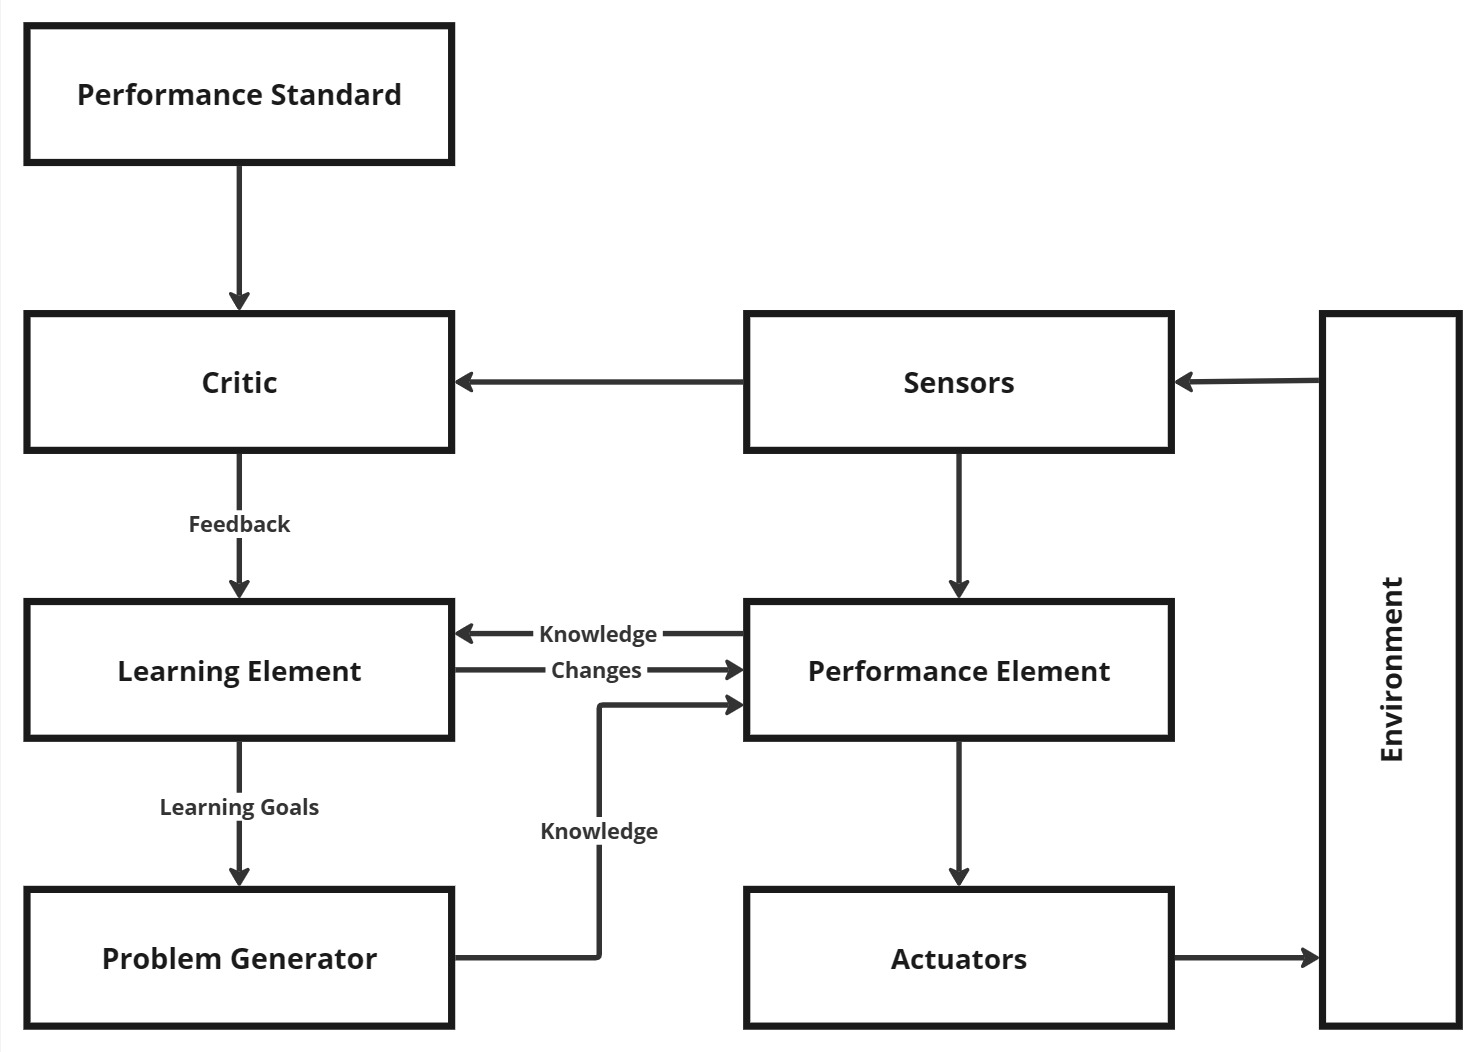
\includegraphics[width=0.5\linewidth]{images/Learning Agent.jpg}
    \caption{Learning Agent}
    \label{fig:learning_agent}
\end{figure}

\subsection{Objective}
There are three main types of artificial intelligent systems:
\begin{itemize}
    \item \textbf{Weak}: an intelligent system that can perform as well as humans. It does not care about the way it achieves the goal, it only focuses on performance.
    \item \textbf{String}: an intelligent system that works by replicating how humans think. It aims to consciously think, not just simulating it.
    \item \textbf{General}: an intelligent system that can solve an arbitrary wide variety of problems, including novel ones, performing as well as humans. 
\end{itemize}
We will focus on weak intelligent systems.

\clearpage
\section{Solving Problems by Searching}
In order to analyze problem solving agents we will consider the simplest of environments only: episodic, single agent, fully observable, static, deterministic, discrete and known.

\subsection{Problem Solving Agents}
Any problem solving agent follows a process divided in four phases:
\begin{enumerate}
    \item \textbf{Goal formulation}: the agent adopts the goals. A goal is useful to organize behavior by limiting the objectives and hence the actions to be considered.
    \item \textbf{Problem formulation}: the agent devises a description of the states and actions necessary to reach the goal. This description is an abstract model of the relevant parts of the world.
    \item \textbf{Search}: before taking any action, the agent simulates sequences of actions in its model, searching until it finds a sequence that reaches the goal. Such a sequence of actions is called a \textbf{solution}. The agent may simulate multiple sequences that do not reach the goal, but eventually it will find a solution, or it will find that no solution is possible.
    \item \textbf{Execution}: the agent executes the actions found in the solution sequence.
\end{enumerate}

\noindent
A search problem can be defined as follows:
\begin{enumerate}
    \item A set of states in which the environment can be in, called the \textbf{state space}, which can be represented as a graph in which the vertices are the states and the directed edges between them are the actions the agent can perform. 
    \item The initial state the agent starts in.
    \item A set of one or more goal states.
    \item The actions available to the agent in a given state. Given a state \textit{s}, the function \code{ACTION(s)} return a finite set of actions the agent can perform in the given state. Such state are called \textbf{applicable} in \textit{s};
    \item A transition model, which describes what each action does. The function \code{RESULT(s, a)} returns the state in which the agent will transition to performing action \textit{a} from state \textit{s}.
    \item An action cost function, denoted by the \code{ACTION-COST(s, a, s')} function, which returns the numeric cost of performing action \textit{a} in state \textit{s} to reach state \textit{s'}. A problem solving agent should use a cost function that reflects its own performance measure.
\end{enumerate}

A solution is a path, which is a sequence of actions, that leads form the initial state to a goal state. The total cost of a path is the sum of the individual costs of every action in the path. An \textbf{optimal solution} is the one that has the lowest path cost among all solutions. 

The formulation of the problem is called \textbf{model}, which is an abstract mathematical description of the problem. The first issue we encounter is that it is usually impossible to represent explicitly the entire state space, because of time and memory limitations, so we must simplify the representation as much as possible. In other words, a problem-solving agent must find a solution by exploring only a small portion of the state space. The process of removing irrelevant details from a representation is called \textbf{abstraction}. The abstraction is valid if we can elaborate any abstract solution into a solution in the more detailed world, and it is useful if carrying out each of the actions in the solution is easier than the original problem. A good abstraction involves removing as much details as possible while retaining validity and ensuring that the abstract actions are easy to carry out.

\subsection{Search Algorithms}
A search algorithm takes a search problem as input and returns a solution. Most of search algorithms are based on a \textbf{search tree data structure} superimposed over the state graph, following various path from the initial state trying to find the one that reaches the goal state. Each node in the search tree corresponds to a state in the state space, while the edges of the tree correspond to actions, as seen in the state graph. The root of the tree corresponds to the initial state of the problem. 

The state space describes the possibly infinite set of states in the world and the actions that allow transitions from one state to another. The search tree describes paths between these states, reaching towards the goal. The search tree may have multiple paths to any given state, but each node has a unique path back to the root of the tree. 

The search tree is created by \textbf{expanding} every node considering the available actions for that state. To do so, we can use the \code{RESULT} function to see where those actions lead to, and generating a new node for each of the resulting states. Now, the algorithm must choose which of these child nodes to consider in order to further expand the tree. This is the core of different search algorithms: they differ from each other for the way they choose the next child to expand in the tree. The set of states that haven't yet been expanded is called \textbf{frontier}, which separates the state space graph into two regions:
\begin{itemize}
    \item The region of states that have been analyzed and thus expanded.
    \item The region of states that haven't yet been expanded.
\end{itemize}

\subsubsection{Best-First Search}
A general approach for deciding which node to expand from the frontier is the \code{BEST-FIRST-SEARCH}, in which we choose a node \textit{n} with minimum value of some evaluation function $f(n)$. On each iteration we choose a node of the frontier with the minimum value of $f(n)$, return it if its state is the goal state, or call the \code{EXPAND} function to generate its child nodes. Each child node is added to the frontier if it has not been reached before, or is re-added if it is reached by a path with a lower costing path. The algorithm returns either an indication of failure if a path is not found, or a node that represents a path to a goal. By using different $f(n)$ functions, we obtain different search algorithms.

\begin{figure}[h]
    \centering
    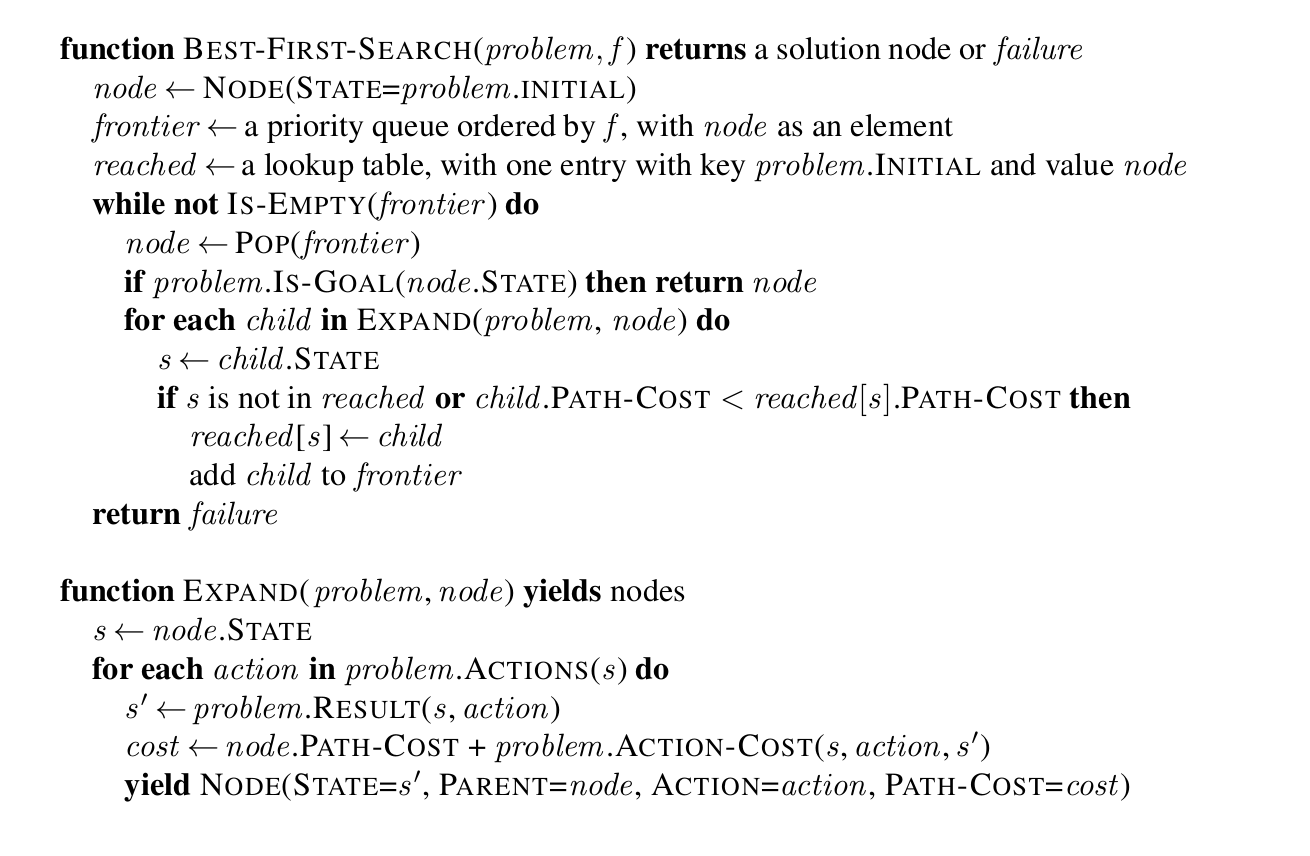
\includegraphics[width=1\linewidth]{algorithms/Best First Search.png}
    \label{fig:best_first_search_algorithm}
\end{figure}

\subsubsection{Search Data Structures}
A node in the search tree is represented by a data structure that requires four components:
\begin{enumerate}
    \item \code{node.STATE}: the state to which the node corresponds.
    \item \code{node.PARENT}: the node in the tree that generated this node.
    \item \code{node.ACTION}: the action applied to the parent node's state to generate this node.
    \item \code{node.PATH-COST}: the total cost of the path from the initial state to this node.
\end{enumerate}

Following the \code{PARENT} pointers back from a node, allows to recover the states and actions along the path to that node. Doing so from a goal node to the root of the tree we obtain the solution to the problem we are analyzing. 

Also a data structure to store the frontier is needed. Different data structures make up different types of searching algorithms. The main ones are:
\begin{itemize}
    \item Priority queue: pops the node with the minimum cost according to some evaluation function.
    \item Queue: pops the first node added to the queue.
    \item Stack: pops the last node added to the stack.
\end{itemize}

The reached states can be stored in a hash table, where each key is a state and each value is a node.

\subsubsection{Redundant Paths}
In the search tree might be repeated states, generated by a cycle (called a loopy path) in the graph over which the tree data structure was superimposed. So, there may be cases where the state space ha a finite amount of states, but the complete search tree is infinite, because there are no limits on how many times a path can be traversed in a loop. This kind of paths are called \textbf{redundant paths}, which represent an obstacle in solving the search related problems. 

If we can eliminate redundant paths, we can make the searching algorithm order of magnitude faster. There are three main approaches to this issue:
\begin{enumerate}
    \item We can store all the previous traversed states in a separate data structure and detect redundant paths in order to keep only the best paths for each state. This approach is appropriate for state spaces where there are many redundant paths and the table of reached states fits in memory.
    \item We can not worry about repeating paths: in some problems is rare or even impossible for two paths to reach the same state, so we can save memory by not tracking reached states and redundant paths. We call a search algorithm a \textbf{graph search} if it checks for redundant paths and \textbf{tree-like search} if it does not.
    \item We can compromise and check only for cycles, but not for redundant paths in general. Since each node has a pointer to its parent node, we can check for cycles simply by following the chain of parents and verify if we land on the same state twice.
\end{enumerate}

\subsubsection{Performance}
An algorithm's performance can be evaluated in three main ways:
\begin{enumerate}
    \item \textbf{Completeness}: whether or not the algorithm is guaranteed to find a solution when there is one and to correctly report failure when there are no solutions.
    \item \textbf{Cost optimally}: whether or not the algorithm finds the most optimal solution, thus the path with the lowest cost of all solutions.
    \item \textbf{Time and Space complexity}: how long does the algorithm take to find a solution and how much memory does it need.
\end{enumerate}

To be complete, a search algorithm must also be \textbf{systematic} in the way it explores an infinite state space, making sure it can eventually reach a goal state which is connected to the initial state. 

The complexity of a search algorithm can be measured in terms of the following parameters:
\begin{itemize}
    \item $d$ - depth: the number of actions in an optimal solution.
    \item $m$: the maximum number of actions in any path.
    \item $b$ - branching factor: the number of successors of a node that need to be considered. 
\end{itemize}

When the branching factor is high, the number of nodes grows quickly and so does the problem complexity. When the depth is large, the closest solution requires more exploration of the search tree, making the algorithm slower.

\subsection{Uninformed Search Strategies}
In uninformed search algorithms no clue is given about how close a state is to the goal and only the information contained in the formulation of the problem itself is used.

\subsubsection{Breadth-First Search}
When all actions inside the state space have the same cost, an appropriate strategy would be a breadth-first search, in which the root node is expanded, then all its successors are expanded next, then their successors and so on. This algorithm is systematic and is therefore complete even on infinite states spaces.

One implementation of this strategy repeatedly calls the \code{BEST-FIRST-SEARCH} algorithm where the evaluation function $f(n)$ is the depth of the node. However, a more efficient implementation would be with a FIFO queue, giving us the correct order of nodes: new nodes (which are deeper than their parents) go to the back of the queue, and old nodes get expanded first, as they are shallower than the new nodes.

Breadth first search always finds a solution with the minimal number of actions, because when it is generating nodes at depth \textit{d}, it has already generated all the nodes at depth \textit{d}-1: if one of them were a solution, it would have been found and the algorithm would have terminated. This means that it is cost optimal for problems where all the actions have the same cost.

\clearpage
\begin{figure}[h]
    \centering
    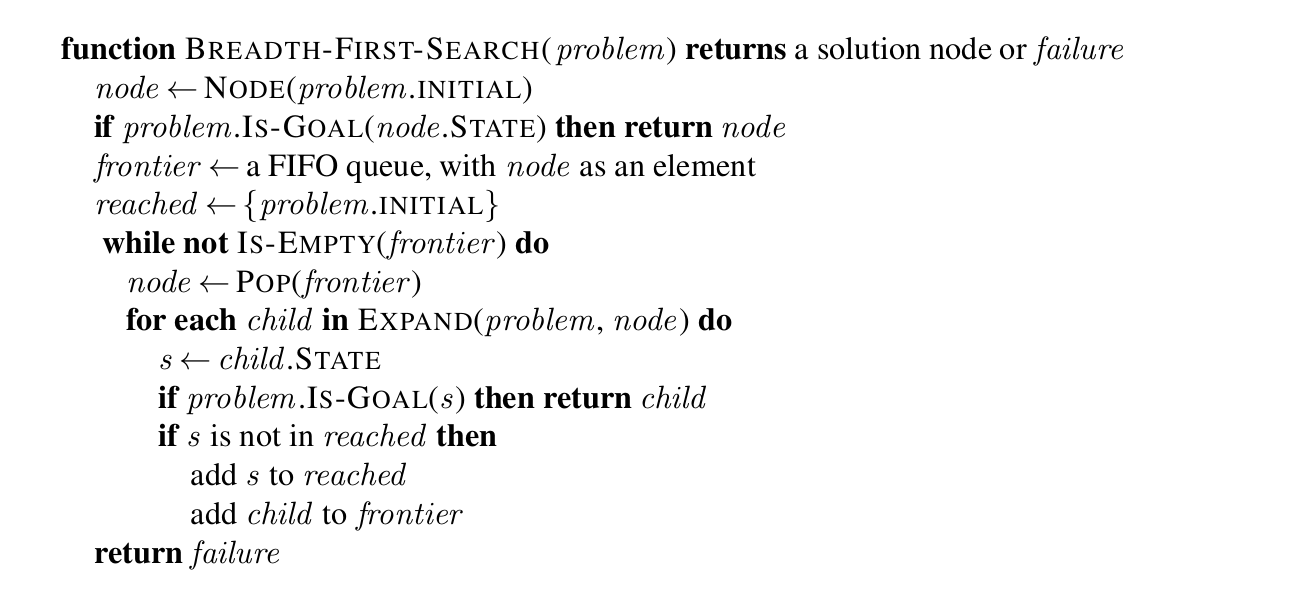
\includegraphics[width=1\linewidth]{algorithms/Breadth First Search.png}
    \label{fig:breadth_first_search_algorithm}
\end{figure}

In order to calculate time and space complexity, we imagine that all nodes in the tree have \textit{b} successors. In this case, the root of the tree generates \textit{b} nodes, each of which generates \textit{b} more nodes, obtaining $b^2$ nodes for the second level. Each of these generates \textit{b} more nodes, yielding $b^3$ nodes at the third level and so on. All these generated nodes remain in memory, so both time and space complexity are $O(b^d)$.

\subsubsection{Uniform-Cost Search}
When actions in the state space have different costs, an obvious choice would be to apply the \code{BEST-FIRST-SEARCH} algorithm, where the evaluation function is the cost of the path from the root to the current node. This type of search is called \textbf{uniform cost search}. The idea behind this type of algorithm is to expand the nodes in waves of uniform path-cost, instead of uniform depth as in the breadth-first search.

\begin{figure}[h]
    \centering
    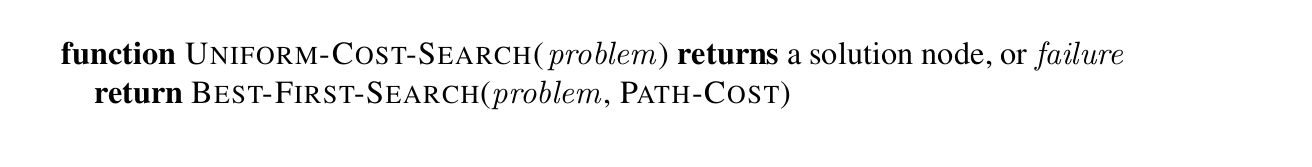
\includegraphics[width=\linewidth]{algorithms/Cost Uniform Search.png}
    \label{fig:uniform_cost_search_algorithm}
\end{figure}

The complexity of this algorithm is characterized in terms of $C^*$, which is the cost of the optimal solution, and $\varepsilon > 0$, which is a lower bound on the cost of each action. Then the algorithm's worst case time and space complexity is $O(b^{1+\lfloor C^*/\varepsilon \rfloor})$, which can be much grater than the $O(b^d)$ found for the breadth-first search algorithm. This is because uniform-cost search can explore very large trees of low-cost actions, before analyzing high-cost and perhaps useful actions. Moreover, the uniform-cost search algorithm is complete and cost-optimal, because the first solution it finds will have a cost that is at least as low as the cost of any other node in the frontier.

\subsubsection{Depth-First Search}
This algorithm always expands the deepest node in the frontier list. The search proceeds immediately to the deepest level of the search tree, where the nodes have no successor. Then, if the goal state is not reached, it "backs up" to the next deepest node that still has unexpanded successors. 

It can be implemented using the \code{BEST-FIRST-SEARCH} algorithm, where the evaluation function is the negative of the depth of the node. Alternatively can be implemented using a LIFO queue (also called stack) to represent the frontier: the generated successor nodes are inserted at the front of the frontier and the most recently generated nodes are selected first.

The depth-first search algorithm is not cost-optimal, as it returns the first solution it finds, even if it is not the cheapest one. For finite state spaces that are trees, it is efficient and complete, but in cyclic state spaces it can get stuck in an infinite loop. For this reason, some implementations of this algorithm check for loops for each new node in the frontier. Finally, for infinite spaces, it is not systematic either, because it can get stuck in infinite path that are not cycles. Thus, depth-first search is incomplete.

Although it has some harsh downfalls, the depth-first search is generally used for its very limited memory usage: this algorithm has much smaller needs for memory, as it doesn't keep track of the reached states at all and it has a small frontier to save in memory. In fact, the depth-first search algorithm has a time complexity of only $O(b\cdot m)$, where $b$ is the branching factor and $m$ is the maximum depth of the tree.

\subsubsection{Depth-Limited Search \& Iterative Deepening Search}
We can prevent the depth-first search algorithm to go on endless paths by limiting the depth at which the algorithm can go. We call this algorithm \textbf{depth-limited search}, with limit $\ell$: we treat all nodes at that depth as if they had no successor. The time complexity of this algorithm is $O(b^\ell)$ and the space complexity is $O(b\ell)$. Unfortunately, if we choose an inappropriate value of $\ell$, the algorithm will fail to reach a solution and it becomes incomplete again. Sometimes a good depth limit can be chosen based on the problem we are trying to solve, but for most problems we will not know a good depth value until we solve the problem.

\textbf{Iterative deepening search} solves the problem of finding a good value for $\ell$ by trying all values until a solution is found or no solutions were found. This approach combines benefits from the depth-first search and breadth-first search algorithms. In fact, like depth-first search, the memory required is modest, spanning from $O(b d)$ when there is a solution, to $O(b m)$ on finite state spaces with no solutions. Like breadth-first search, iterative deepening search is optimal for problems where all the actions have the same cost, and is complete on finite acyclic state spaces, or on any finite state space when we check nodes for cycles all the way up the path. The time complexity is $O(b^d)$ when there is a solution, or $O(b^m)$ when there is none.

\begin{figure}[h]
    \centering
    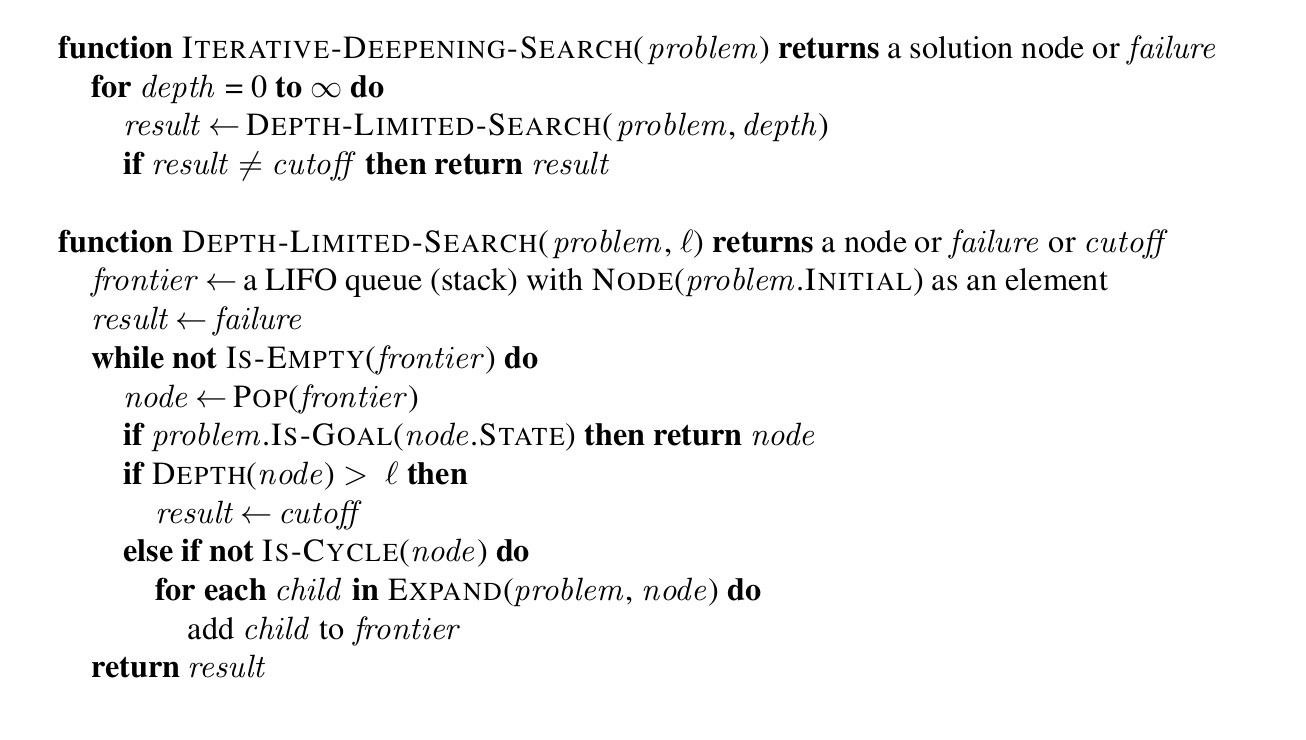
\includegraphics[width=1\linewidth]{algorithms/Iterative Deepening and Limeted Search.png}
    \label{fig:iterative_deepening_and_limited_search_algorithms}
\end{figure}

\subsubsection{Bidirectional Search}
One last strategy we can apply for uninformed search can be to go backward, from the solution to the initial state if the problem is easily reversible. A more efficient way is to combine the two directions into a bidirectional search: this type of search performs two searches in parallel, one \textit{forward} search from the initial state to the goal state, one \textit{backwards} search from a goal state to the initial state.

\subsubsection{Summary}

Tree search algorithms work well when the the state space is represented as a tree-like data structure, while graph search algorithms work well with graphs. For each algorithm analyzed so far, several variants are possible, but there are always trade-offs between memory usage for storing the closed list and the time spent to check it.


The following tables compare the characteristics of the main algorithms analyzed so far, where:
\begin{itemize}
    \item $b$: number of successors of a node that need to be considered;
    \item $d$: number of actions in an optimal solution;
    \item $m$: maximum number of actions in any path;
    \item $C^*$: cost of the optimal solution;
    \item $\varepsilon$: lower bound on the cost of each action;
    \item $\ell$: depth limit;
\end{itemize}
\begin{table}[h]
    \begin{tabular}{lcccc}
        \multicolumn{1}{l}{} & \multicolumn{2}{c}{\textit{With repeated states}} & \multicolumn{2}{c}{\textit{Without repeated states}} \\
        \multicolumn{1}{r||}{Search Strategy} & \multicolumn{1}{c|}{Complete} & \multicolumn{1}{c|}{Optimal} & \multicolumn{1}{c|}{Complete} & Optimal \\ \hline \hline
        \multicolumn{1}{l||}{\textbf{Breadth-First Search}} & \multicolumn{1}{c|}{YES} & \multicolumn{1}{c|}{YES} & \multicolumn{1}{c|}{YES} & YES \\ \hline
        \multicolumn{1}{l||}{\textbf{Uniform-Cost Search}} & \multicolumn{1}{c|}{YES} & \multicolumn{1}{c|}{YES} & \multicolumn{1}{c|}{YES} & YES \\ \hline
        \multicolumn{1}{l||}{\textbf{Depth-First Search}} & \multicolumn{1}{c|}{NO} & \multicolumn{1}{c|}{NO} & \multicolumn{1}{c|}{YES} & NO \\ \hline
        \multicolumn{1}{l||}{\textbf{Limited-Depth Search}} & \multicolumn{1}{c|}{NO} & \multicolumn{1}{c|}{NO} & \multicolumn{1}{c|}{NO} & NO \\ \hline
        \multicolumn{1}{l||}{\textbf{Iterative Deepening}} & \multicolumn{1}{c|}{YES} & \multicolumn{1}{c|}{YES} & \multicolumn{1}{c|}{YES} & YES
    \end{tabular}
    \caption{Strategy comparison}
    \label{tab:strategy_comparison}
\end{table}

\begin{table}[h]
    \centering
    \begin{tabular}{l||c|c}
        Strategy & S(n) & T(n) \\ \hline \hline
        \textbf{Breadth-First Search} & $O(b^d)$  & $O(b^{d+1})$ \\ \hline
        \textbf{Uniform-Cost Search} & $O(b^{1+\lfloor C^*/\varepsilon \rfloor})$ & $O(b^{1+\lfloor C^*/\varepsilon \rfloor})$ \\ \hline
        \textbf{Depth-First Search} & $O(bm)$ & $O(b^m)$ \\ \hline
        \textbf{Limited-Depth Search} & $O(b\ell)$ & $O(b^\ell)$ \\ \hline
        \textbf{Iterative Deepening} & $O(bd)$ & $O(b^d)$ \\
    \end{tabular}
    \caption{Strategy Complexity}
    \label{tab:strategy_complexity}
\end{table}

\subsection{Informed Search Strategies}
In informed search algorithms, specific knowledge that is not contained in the problem formulation is exploited to solve the problem itself. This strategy selects a node from the frontier according to an evaluation function $f(n)$, which provides an estimate of how much a node is "promising". There are two main ways of calculating the evaluation function:
\begin{enumerate}
    \item Greedy best-first search.
    \item A* search.
\end{enumerate}

Conventionally, the most promising nodes have a small value of the evaluation function $f(n)$, so the frontier is implemented as a priority queue ordered in increasing order of $f(n)$. Thus, nodes with the minimum $f(n)$ are chosen first.

\subsubsection{Greedy Best-First Search}
Greedy best-first search algorithms use an evaluation function that is equal to the \textbf{heuristic function} $h(n)$, which gives the \textit{estimated} cost of the cheapest path from the state at node $n$ to a goal state. To apply the greedy best-first search, the function $h(n)$ must be known. Note that, the heuristic is an estimate, not an actual cost: if we knew the actual cost of the path, the problem would have already been solved.

There are many heuristic functions we can choose for every given problem, but there are some more accurate than others. In fact, given two heuristic functions $h_1(n)$ and $h_2(n)$, such that $h_1(n)\le h_2(n)$ for any node $n$, $h_2$ is said to dominate $h_1$ since each node expanded using $h_2$ is also expanded using $h_1$. In this case we say that the function $h_2$ is more accurate, or more informed, than the function $h_1$.

Greedy best-first search is neither complete nor optimal, as it can get stuck in local optimal solutions, without the possibility of backtracking, or in infinite loops. The time and space complexity of this algorithm in the worst-case scenario are both $O(b^m)$, where $m$ is the maximum depth of the search tree (which could be infinite).

\subsubsection{A* Search}
The most used informed search algorithm is \textbf{A* search}, a best-first search that uses the evaluation function $f(n) = g(n) + h(n)$, where:
\begin{itemize}
    \item $g(n)$ is the path cost from the initial state to node $n$. This function is known.
    \item $h(n)$ is the estimate cost of the shortest path from $n$ to a goal state. This function is estimated.
\end{itemize}

\noindent
In other words, $f(n)$ is the estimated cost of the best path that continues from the state $n$ to a goal state. By using both the cost so far and the estimated cost of reaching the goal, A* can lead the agent away from suboptimal paths.

A* search is complete and optimal for tree-search when the function $h(n)$ is \textbf{admissible}. A heuristic function is admissible when, for each node $n$, it is true that 
    $$0 \le h(n) \le h^*(n)$$
where $h^*(n)$ represents the actual cost from the given node to a solution node. When $n$ is a goal state, $h(n)$ should be zero. An admissible heuristic is \textit{"optimistic"} since it always underestimates the true cost to reach the goal. In fact it can be seen as the cost of an optimal solution to a relaxed problem, obtained by removing the constraints.

A* search is also complete and optimal for graph-search when the function $h(n)$ is \textbf{consistent}. An heuristic function is consistent when, for every node $n$ and every successor $n'$ generated from $n$ by action $a$, it is true that 
$$h(n)\le c(n,a,n') + h(n') \;\; \textnormal{(triangular inequality)}$$
When $n$ is a goal state, $h(n)$ should be zero. Every consistent heuristic function is also an admissible one, but not vice versa. Consistency is a stronger property than admissibility, because graph-search is more constrained since it does not consider nodes corresponding to the same state, thus it requires a stronger property to guarantee completeness and optimality. In addition, with a consistent heuristic, the first time we reach a state it will be on an optimal path, so we never have to re-add a state to the frontier and never have to change an entry in the \textit{reached} set.

There are many types of consistent heuristic functions, but some of them are uninteresting: for example, the heuristic function $h_0(n) = 0 \;\; \forall n$ is consistent and admissible, but it implements a uniform-cost search (uninformed search algorithm), so it is not really that interesting.

A special variation of the A* search is the \textbf{weighted A* algorithm}. It introduces a weight factor $w$, which is $1 \le w < \infty$, over the heuristic functions so that $f(n) = g(n) + w \cdot h(n)$. The theoretical properties of the simple A* search do not apply anymore, but this extension of the algorithm can be more efficient and solve search problems quicker.

The last, and most successful, variation of A* search is the \textbf{iterative-deepening A* search} (IDA* search), which reduces memory requirements by applying a limit to the values of the evaluation function $f(n)$. It is to A* what iterative-deepening was to depth-first search: IDA* gives all the benefits of A* without the requirement to keep the reached states in memory, at the cost of visiting some states multiple times. In IDA* the cutoff value is the $f-cost (g+h)$; at each iteration, the cutoff value is the smallest $f-cost$ of any node that exceeded the cutoff on the previous iteration. IDA* search is complete and optimal when the heuristic function $h(n)$ is admissible.

\clearpage
\section{Constraint Satisfaction Problems}
In standard search, the basic idea is that problems can be solved by searching the state space, that is a graph in which nodes represent states and edges between them represent actions. In this type of search algorithms, the states are atomic, indivisible, like a \textit{black box}: for each problem, we need domain-specific heuristic function to describe the transition between states.

In \textbf{constraint satisfaction problems}, \textbf{CSP} for short, we break open this black box by using a factored representation for each state, that consists of a set of variables, each of which have a value. A CSP is solved if each variable has a value that satisfies all the constraints on that variable.

CSP search algorithms take advantage of the structure of states and use a general heuristic to enable the solution of complex problems. The main idea is that we can eliminate large portions of the search space by identifying values that violate constraints on variables. A CSP consists of three components:
\begin{itemize}
    \item $\mathcal{X} =\{X_1, ..., X_n\}$ is a set of variables;
    \item $\mathcal{D} =\{D_1, ..., D_n\}$ is a set of domains, one for each variable;
    \item $\mathcal{C}$ is a set of constraints that specify valid combinations of values.
\end{itemize}

A domain $D_i$ is a set of allowable values $\{v_1, ..., v_k\}$ for each variable $X_i$. Each constraint $\mathcal{C}_j$ consists of a pair $\langle scope,\; rel\rangle$, where $scope$ is a tuple of variables that participate in the constraint, and $rel$ is a relation that defines the valid values for those variables. A relation can be represented as an explicit set of all tuples of values that satisfy the constraint, or as a function that can compute whether or not a tuple is a member of the solution.

The goal of the CSP is to assign values to the variables, such that 
    $$\{X_i=v_i, X_j=v_j, ...\}.$$ 
An assignment is \textbf{consistent} if does not violate any constraints and is \textbf{complete} if all variables are assigned a value. A solution to a CSP is a consistent and complete assignment. If all the domains have fixed size $d$, there are $O(d^n)$ complete assignments possible.

Every CSP can be visualized as a constraint graph: the nodes of the graph correspond to variables of the problem and the edge connects any two variables that participate in a constraint. This type of representation for the problem can dramatically speed up the search problem, by showing that some variables are independent sub-problems. Additionally, we will consider only binary constraints, in which only two variables are involved, because higher order constraints can be transformed in a CSP with only binary constraints through simple transformations.

\subsection{Constraints Propagation - Arc consistency}
A variable in a CSP problem is arc-consistent if every value in its domain satisfies the variable's binary constraints. More formally, $X_i$ is arc-consistent with respect to another variable $X_j$ if there is some value in the domain $D_j$ that satisfies the binary constraint in the arch $(X_i, X_j)$. In other words, arc consistency is a property that allows to remove from the domain of a variable $X$ every value that is inconsistent with the values in the domain of another variable $Y$. 

The most popular algorithm for enforcing the arc-consistency property on a CSP problem is called \textbf{AC-3}, which maintains a queue of arcs to consider. Initially, the queue contains all the arcs in the CSP. Then, the algorithm pops off an arbitrary arc $(X_i, X_j)$ and makes $X_i$ arc-consistent with respect to $X_j$. If this leaves $D_i$ unchanged, the algorithm moves on the next arc, but if this operation revises the domain $D_i$ (making it smaller), then we add to the queue all arcs $X_k, X_i$, where $X_k$ is a neighbor of $X_i$. This is necessary because, by reducing $D_i$, we might enable further reductions in $D_k$, even if we've already applied the algorithm to that node. If $D_i$ is revised down to nothing, then we know that the whole CSP problem has no consistent solution and the algorithm can immediately return failure. Otherwise, we keep checking, trying to remove values from the domains of variables until no more arcs are in the queue. At this point we are left with a CSP equivalent to the initial one, but the arc consistent one will be faster to search because its variables have smaller domains. The complexity of AC-3 is $O(cd^3)$ in the worst case scenario.

\begin{figure}[h]
    \centering
    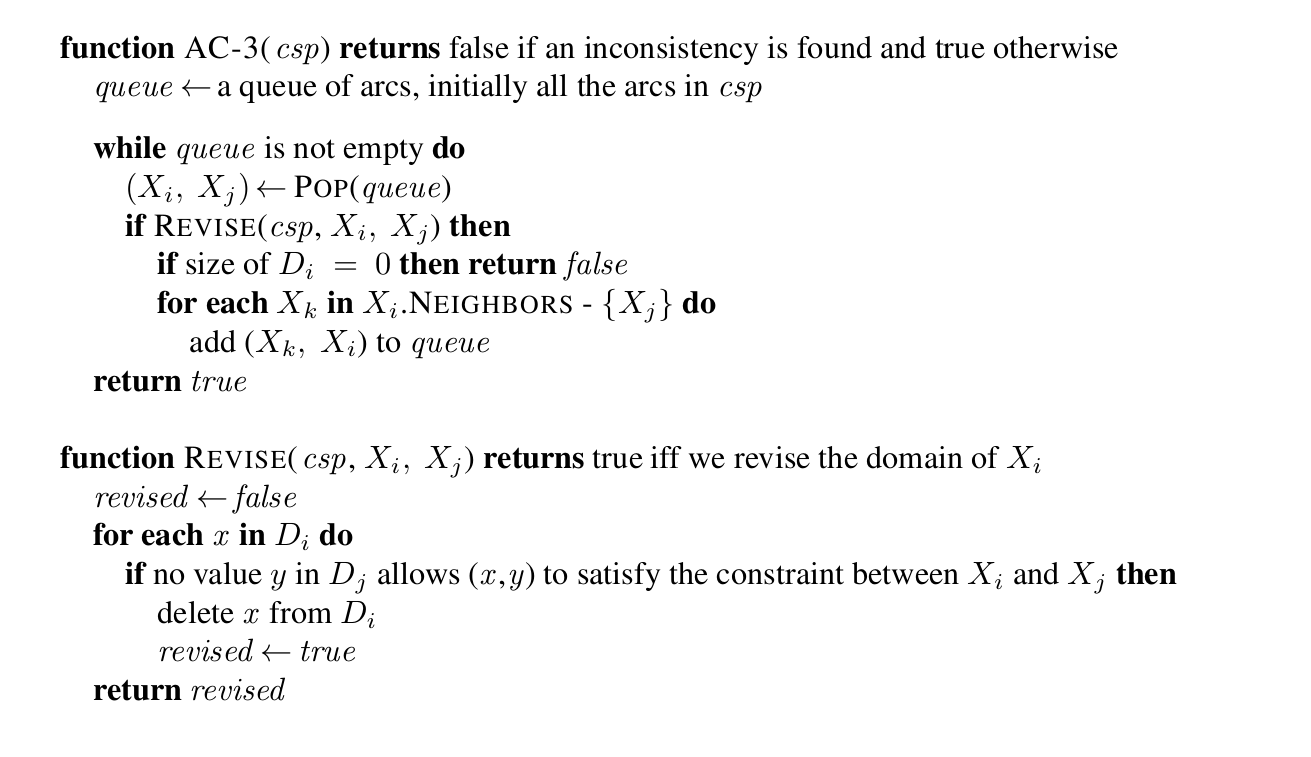
\includegraphics[width=1\linewidth]{algorithms/AC-3.png}
    \label{fig:ac_3_algorithm}
\end{figure}


\subsection{Backtracking Search for CSP}
Sometimes we can finish the constraint propagation process and still have variables with multiple possible values. In this case we have to search a solution. For a CSP problem with $n$ variables of domain size $d$ we would end up with a search tree where all the complete assignments are leaf nodes at depth $n$. But, the branching factor at the top level would be $nd$ because any of $d$ values can be assigned to any of $n$ variables. At the next level, the branching factor is $(n-1)d$ and so on for $n$ levels. So the tree has $n!d^n$ leaves, even though there are only $d^n$ possible assignments.

We can remove the $n!$ factor by recognizing that CSP have the \textbf{commutative property}. A problem is said to be commutative if the order of any given set of actions does not matter. In CSPs it makes no difference if we first assign a value to a variable and then to another, or the other way around. Therefore, we need only to consider a single variable at each node in the search tree. At each level of the tree we must choose which variable we will deal with, but we never have to backtrack over that choice. 

\begin{figure}[h]
    \centering
    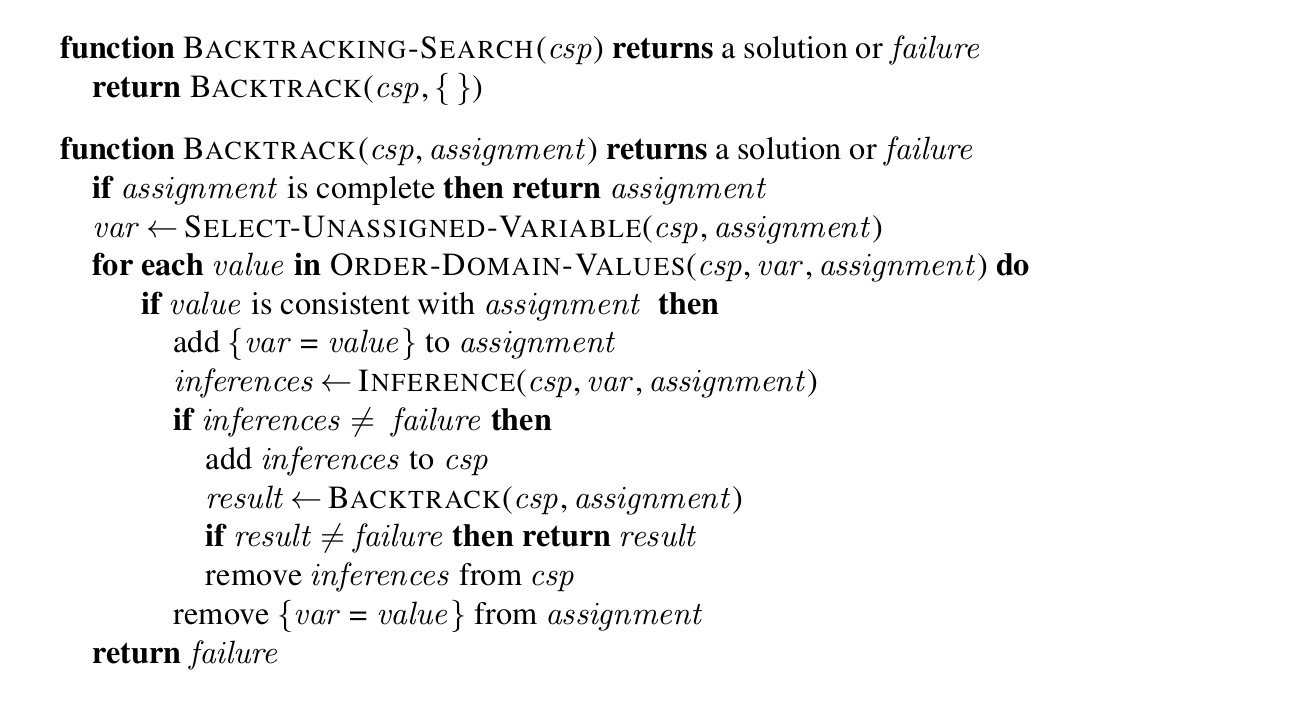
\includegraphics[width=1\linewidth]{algorithms/Backtracking Search for CSP.png}
    \label{fig:backtracking_search_for_CSP_algorithm}
\end{figure}

Backtracking search algorithm for CSP repeatedly chooses an unassigned variable and tries all values in the domain of that variable in turn, trying to extend each one into a solution recursively. If the call succeeds, the solution is returned, otherwise the assignment is restored to the previous state, from which we try all the remaining values. If no value works we return a failure. This algorithm can be improved by using domain-independent heuristics that take advantage of the factored representation of the CSP. The functions \code{SELECT-UNASSIGNED-VARIABLE} and \code{ORDER-DOMAIN-VALUES} are the heart of the backtracking algorithm, which implement a general purpose heuristics. Also, the \code{INFERENCE} function is really important, as it simplifies the problem by relaxing some constraints.

\subsubsection{Variable ordering}
There are various strategies we can implement in order to select an unassigned variable. The simplest one is to choose variables in order or randomly. There are better heuristics, like choosing the variable with the fewest possible values, called \textbf{minimum-remaining-values} (\textbf{MRV}). This strategy is also called "fail-first" as it picks a variable that is most likely to cause a failure soon, thereby pruning the tree.

Another strategy is the \textbf{degree heuristic}, which attempts to reduce the branching factor on future choices by selecting the variable that is involved in the largest number of constraints on other unassigned variables. The MRV heuristic is usually more powerful, but the degree heuristic can be useful as a tie-breaker, when multiple values can be chosen.

Once a variable is selected, the algorithm must decide on the order to examine its values. An efficient algorithm is the \textbf{least-constraining-value} heuristic, which prefers the value that rules out the fewest choices for the neighboring variables in the constraint graph.

Variables should be selected following the "fail-first" principle, while its values should follow the "fail-last" principle. This is because every variable has to be assigned eventually, so by choosing the ones that are likely to fail first, we will have fewer successful assignments to backtrack over. On the other hand, for value ordering we need only one solution, so it makes sense to look for the most likely values first.

\subsubsection{Forward Checking}
The AC-3 algorithm can reduce the domains of variables before we begin the search, but inference can be more powerful during the search. One simple type of inference is \textbf{forward checking}. Whenever a variable $X$ is assigned, the forward checking algorithm establishes arc consistency for it: for each unassigned variable $Y$ connected to $X$ by a constraint, it deletes from $Y$'s domain any value that is inconsistent with the value chosen for $X$. A problem with forward checking is that although it detects many inconsistencies, it does not detect them all.

Given $n$ variables, the size of the domain $d$ and the largest number of constraint that involve any given variable $s$, such that $s\le n-1$, the complexity of forward checking is $O(snd)$.

\subsection{Local Search}
We can efficiently solve CSPs using another paradigm: \textbf{local search}. It uses a complete state formulation where each state assigns a value to every variable, and the search changes the value of one variable at a time. In other words, it starts from a random solution and modifies it a little bit until we reach a feasible solution. This strategy uses the \textbf{hill-climbing} algorithm to evaluate whether or not the modified solution improves the current one. Considering the states of a problem as laid out in a state-space landscape, each point has an "elevation", defined by the value of the objective function; the problems is narrowed down to finding the global maximum value. The only problem in this kind of algorithms is that they can stop at local maxima, yielding a sub-optimal solution.



\clearpage
\section{Adversarial Search and Games}
Adversarial search problems are a set of problems in which we explore competitive environments, where two or more agents have conflicting goals.

\subsection{Two-Player Zero-Sum Games}
The most studied problems in AI are the deterministic, two-player, turn-taking, perfect information (fully observable) and zero-sum (there's always one winning player) games. In game theory the terms \textbf{move} and \textbf{position} are used as synonym for action and state respectively. Games can be formulated as a search problem with an element of uncertainty due to the actions taken by the opponent. In this case, there is no sequence of moves that makes a player win no matter the actions taken by the opponent. At each turn, each player must choose an action without the possibility of exploring the whole state space.

The analyzed games will always involve two players, called \code{MAX} and \code{MIN}, in which \code{MAX} moves first and then the players take turns moving until the game is over. A game can formally be defined with the following elements:
\begin{itemize}
    \item $S_0$: the initial state, which specifies how the game is set up at the start;
    \item \code{TO-MOVE(s)}: the player whose turn it is to move in state $s$;
    \item \code{ACTIONS(s)}: the set of legal moves the player can do in state $s$;
    \item \code{RESULT(s, a)}: the transition model, which defines the state resulting from the taking action $a$ in state $s$;
    \item \code{IS-TERMINAL(s)}: the terminal test, which returns true if the game is in a terminal state, false otherwise;
    \item \code{UTILITY(s, p)}: the utility function, which defines the final numeric value to player $p$ when the game ends in terminal state $s$.
\end{itemize}

The initial state, the \code{ACTIONS} function and the \code{RESULT} one define the \textbf{state space graph}, where the vertices represent the states and the edges the moves. As always a \textbf{search tree} can be superimposed on the graph (or on a particular part of it), to determine what moves to make next. We can define the complete \textbf{game tree} as the search tree that follows every possible path all the way down to a terminal state, or up to a maximum depth $h$, based on the available space and time. At the beginning, \code{MAX} builds the game tree \textit{from its perspective} using a depth-first search algorithm. Leaf nodes contain the utility value of the terminal state from the point of view of \code{MAX}, calculated via the utility function or by an evaluation function $e(s)$: high values are good for \code{MAX} and bad from \code{MIN}. Solving the game corresponds to finding the best moves for \code{MAX} (or \code{MIN}) in a state.

\subsection{Optimal Decisions}
Given a game tree, the optimal strategy can be determined by evaluating the \textbf{minimax} value of each state of the tree, which is indicated with \code{MINIMAX(s)}. This value is the utility for \code{MAX} being in that state, \textit{assuming that both players play optimally}. The minimax value of a terminal state is just its utility. In any terminal space, \code{MAX} prefers to move to a state of maximum value when it's his turn to move, while \code{MIN} prefers a state of minimum, which is minimum value for \code{MAX} (thus maximum value for \code{MIN}). The \code{MINIMAX} function is calculated as follows:
$$
    minimax(s)=
        \begin{cases}
            utility(s, max)&if\;\;isTerminal(s)\\
            \max_{a\in actions(s)}minimax(result(s,a))&if\;\;toMove(s) = max\\
            \min_{a\in actions(s)}minimax(result(s,a))&if\;\;toMove(s) = min\\        
        \end{cases}
$$

If \code{MIN} does not play optimally, then \code{MAX} will be at least as good as against an optimal player, possibly better.

In some games it is impossible to build the entire game tree because of space limitations, so the the utility function cannot be computed; instead the evaluation function is computed, which gives an estimated value of the expected utility for the player $p$ in a non-terminal state $s$. The evaluation function can yield positive or negative values, where $e(s) > 0$ is good for \code{MAX}, $e(s) < 0$ is good for \code{MIN} and $e(s) = 0$ is neutral, as they are calculated from the perspective of \code{MAX}. The values for \code{MIN} are obtained by taking the opposite of \code{MAX}'s values, as the games are zero sum. Furthermore, the value of $e(s)$ can be normalized between -1 and +1 to keep values consistent with the utility function. Starting from the values assigned to the leaves and going up to the root of the tree, a minimax value is assigned to each node of the game tree. The minimax value of a node is the estimate of the expected utility for a player in the state corresponding to that node, if both players play optimally.

\subsubsection{Minimax search algorithm}
By using the \code{MINIMAX} function, we can build a \textbf{minimax search algorithm} that finds the best move for \code{MAX}, by trying all actions and choosing the one whose resulting state has the highest \code{MINIMAX} value. This algorithm is recursive and proceeds all the way down to the leaves of the tree and than backs up the minimax values through the tree as the recursion unwinds.

\begin{figure}[h]
    \centering
    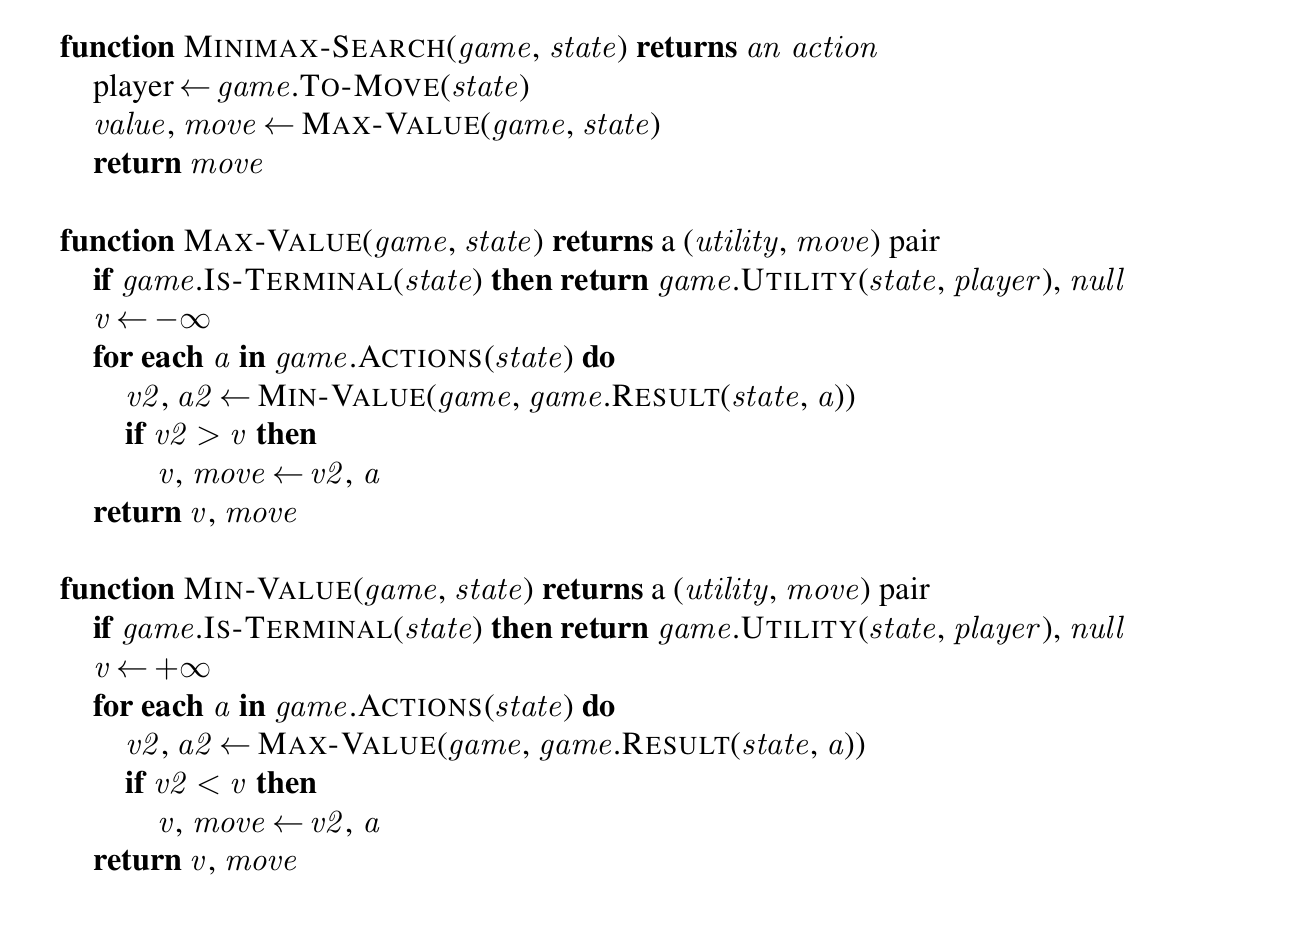
\includegraphics[width=1\linewidth]{algorithms/Minimax.png}
    \label{fig:minimax_algorithm}
\end{figure}

The minimax algorithm is optimal when the entire game tree is built and the utility function can be used. The algorithm performs a complete depth-first exploration of the game tree: if the maximum depth of the tree is $m$ and there are $b$ legal moves at each point, then the time complexity of the minimax algorithm is $O(b^m)$ and the space complexity is $O(bm)$. The exponential time complexity makes the minimax algorithm impractical for complex games. By approximating the analysis in various ways, we can write more efficient algorithms.

\subsubsection{Alpha-Beta pruning}
As seen in the previous section, the number of game states is exponential in the depth of the tree. We can speed up the algorithms by \textbf{pruning} (cutting off) large portions of the tree that make no difference to the outcome. We will examine the \textbf{alpha-beta pruning} technique.

Sometimes the minimax value is independent from the value of other nodes. Let $n$ be a node of the tree, such that the player has a choice of moving to $n$: if the player has a better option either at the same level as $n$ or higher up, the player will never move to $n$. So, once we have found out enough about $n$ to reach this conclusion, we can prune the entire subtree with root in $n$. 

The alpha-beta pruning gets its name from the two extra parameters passed to the \code{MAX-VALUE(}$s, \alpha, \beta$\code{)} function, that describe bounds on the backed-up values that appear anywhere along the path:
\begin{itemize}
    \item $\alpha$ is the value of the best choice we have found so far at any choice point along the path for \code{MAX}. We can think of $\alpha$ as "\textit{at least}".
    \item $\beta$ is the value of the best choice we have found so far at any choice point along the path for \code{MIN}. We can think of $\beta$ as "\textit{at most}".
\end{itemize}

Alpha-beta search updates the values of $\alpha$ and $\beta$ as it goes along and prunes the remaining branches at a node as soon as the value of the current node is known to be worse than the current $\alpha$ or $\beta$ value for \code{MAX} or \code{MIN} respectively.

\begin{figure}[h]
    \centering
    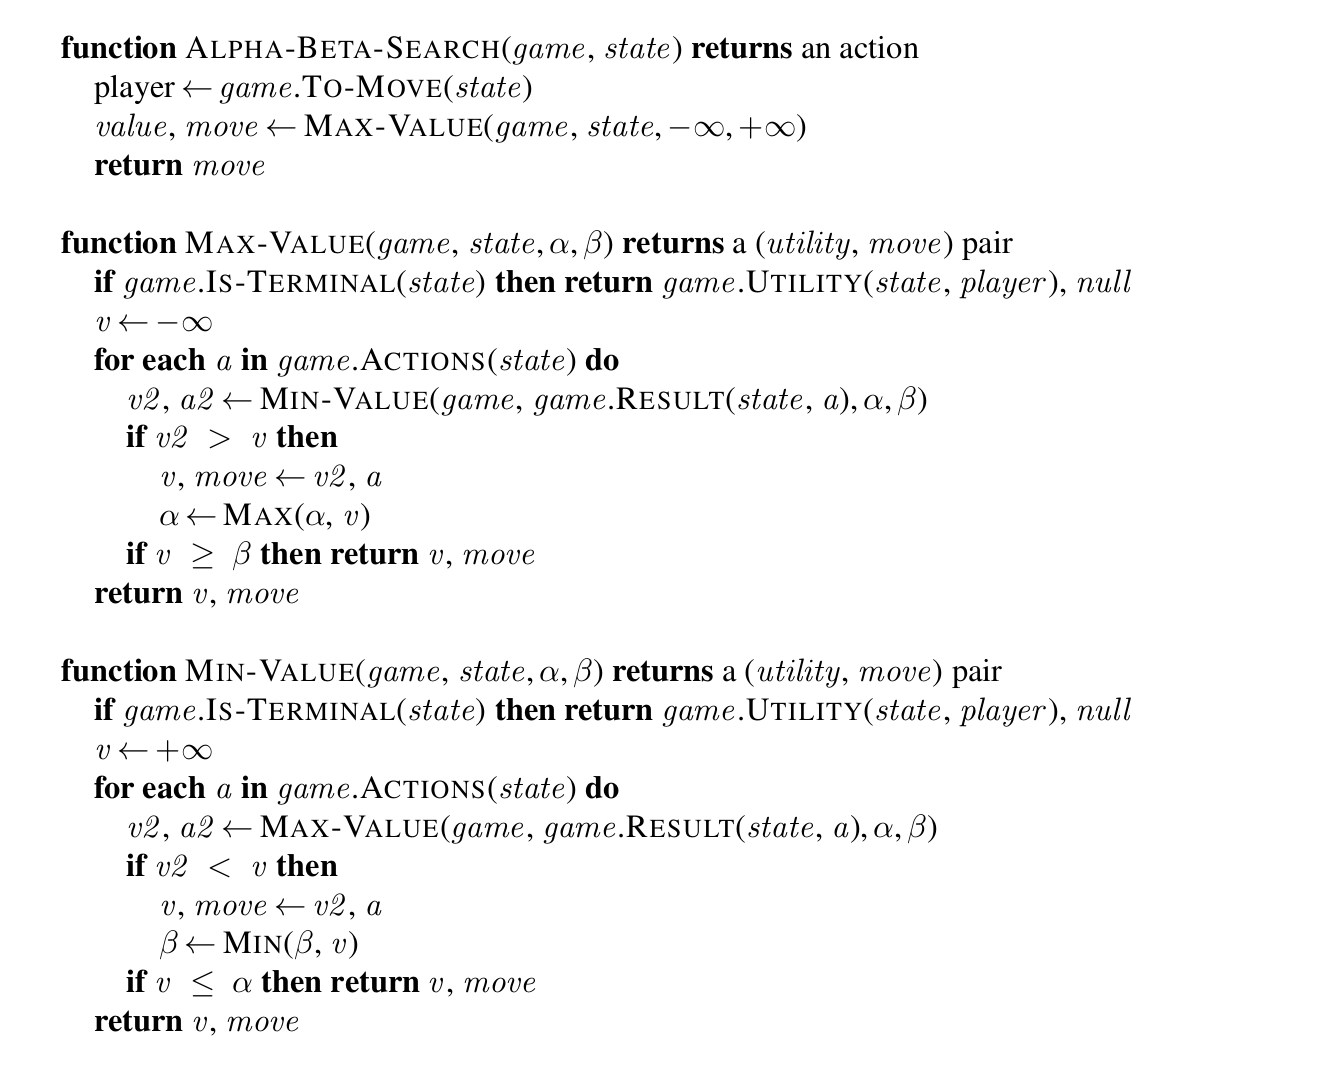
\includegraphics[width=1\linewidth]{algorithms/Alpha Beta Pruning.png}
    \label{fig:alpha_beta_pruning_algorithm}
\end{figure}

In order to make Alpha-beta pruning highly efficient we need to make some clarifications about the order in which we examine the states. One improvement we can make is to examine first the successors that are likely to be best. If this could be done perfectly, alpha-beta pruning would need to examine only $O(b^{m/2})$ nodes to pick the best move, instead of the $O(b^m)$ required by the minimax algorithm. So, alpha-beta pruning with perfect move ordering can solve a tree roughly twice as deep as minimax in the same amount of time. In reality, if the nodes are considered in random order, alpha beta pruning expands on average $O(b^{3h/4})$ nodes, pruning roughly 25\% of the game tree.

Lastly, in game tree search, repeated states can occur because of transpositions, which are different permutations of the move sequence that end up in the same position. These repeated states can cause an exponential increase in search cost. The problem can be addressed with a \textbf{transposition table}, that caches the heuristic values of a state, reducing the time complexity of the alpha-beta pruning algorithm. 

\subsection{Stochastic Games}
Stochastic Games bring us a little closer to the real world by adding a random element in the computation. In this case, the game tree must include \textbf{chance nodes} (represented in circles) in addition to \code{MAX} and \code{MIN} nodes. The branches leading from each chance node denote the random probability. 

In this kind of games, we still want to pick the move that leads to the best decision. However, positions do not have definite minmax values. Instead, we can only calculate the \textbf{expected value} of a position: the average overall possible outcome of the chance nodes. This leads to the \textbf{expectiminimax value} for games with chance nodes, a generalization of the minimax value for deterministic games. Terminal, \code{MAX} and \code{MIN} nodes work exactly the same as before, but for chance nodes we compute the expected value, which is the sum of the value over all outcomes, weighted by the probability of each chance action:
\begin{multline*}
    expectiminimax(s) = \\
    \begin{cases}
        utility(s, max) & if \;\; isTerminal(s) \\
        \max_{a\in actions(s)} expectiminimax(result(s, a)) & if \;\; toMove(s) = max \\
        \min_{a \in actions(s)} expectiminimax(result(s, a)) & if \;\; toMove(s) = min \\
        \Sigma_{r}P(r) expectiminimax(result(s, a)) & if\;\; toMove(s) = chance\\
    \end{cases}
\end{multline*}

Where $r$ represents the chance event and $result(s, r)$ is the same state as $s$, with the additional fact that the outcome of the event is $r$.

\subsection{Monte Carlo Tree Search}
For games with large state spaces and high branching factor the algorithms used up to now are impractical. Furthermore, there are cases in which we don't now the domain very well and the branches are all equally promising. In this cases, the best algorithm to use is the Monte Carlo Tree Search. It does not use a heuristic function to solve the problem, but instead the value of a state is determined as the average utility over a number of simulations of complete games starting from that state. A simulation, also called \textbf{playout} or \textbf{rollout}, chooses moves first for one player, then for the other, repeating until a terminal position is reached. At that point, the rules of the game decide who has won or lost, determining the "win percentage".

In order to get useful information from the playout we need a \textbf{playout policy}, that biases the moves towards good ones instead of randomly choosing between the available ones. Once a policy has been chosen, we need to decide from what position to start the playouts and how many do we need to allocate for each position. The simplest solution is to start from the current state of the game and compute $N$ simulations, tracking down which of the possible moves from the current position has the highest win percentage.

While for stochastic games this converges to optimal play as $N$ increases, for most game it is not sufficient: we need a \textbf{selection policy} that focuses on the important parts of the game tree. It should balance two main factors: exploration of states that have had few playouts, and exploitation of states that have done well in past playouts, to get more accurate estimate of their value.

Monte Carlo Tree Search does that by maintaining a search tree and growing it on each iteration of the following steps:
\begin{enumerate}
    \item \textbf{Selection}: it descends the game tree starting at the root of the search tree, selecting successors using a selection policy until either a node with an unexpanded branch or a leaf node is reached.
    \item \textbf{Expansion}: if the node is not a goal, the tree is expanded by generating one or more children nodes.
    \item \textbf{Simulation}: it performs a playout from the newly generated child node, choosing moves for both players according to the default playout policy. This results in a reward computed according to a reward function.
    \item \textbf{Back-propagation}: the result of the simulation is used to update all the search tree nodes going up to the root.
\end{enumerate}

We repeat these four steps either for a set number of iterations or until the allotted time has expired, and then return the move with the highest number of playouts.

\begin{figure}[h]
    \centering
    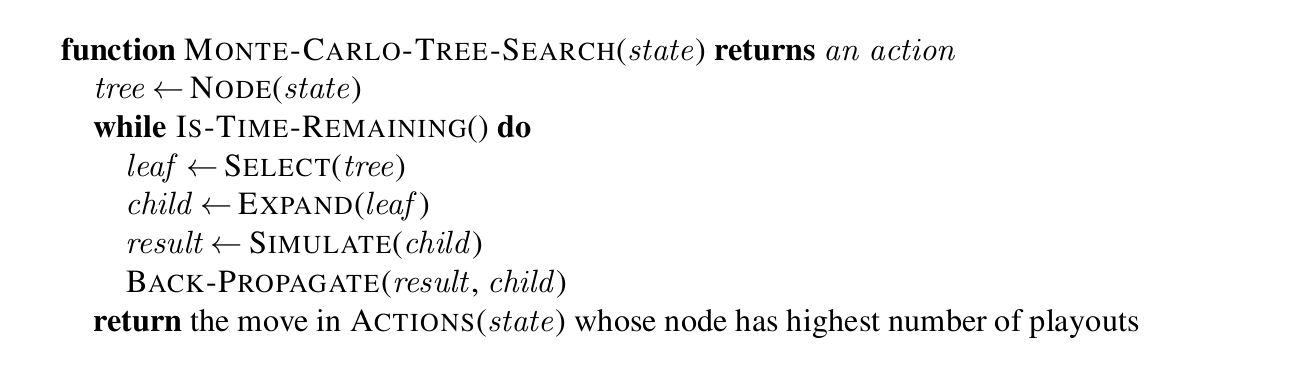
\includegraphics[width=1\linewidth]{algorithms/Monte Carlo Search.png}
    \label{fig:monte_carlo_search_algorithm}
\end{figure}



\noindent Each node $n$ of the Monte Carlo tree stores a pair of values:
\begin{enumerate}
    \item either the number of wins for the player at the root or the number of wins for the player at that node.
    \item the number of performed simulations that involve the node $n$.
\end{enumerate}
In general, the utilities $U(n)$ are stored in each node. 

As already said, the selection policy must be a balance between exploration and exploitation: the agent should visit nodes that promise high chance of winning, but at the same time should try less explored nodes to find new high rewording paths.
We model this as the \textbf{k-armed bandits problem}, in which an agent must decide between $k$ actions and receive a reward based on the action it chooses. More formally, at time $t$, the agent selects an action $a_t$, and receives a reward $R_t$. The goal of the agent is to maximize the following:
    $$\sum_{t=1}^{T}R_t$$
Also, the agent must learn how much it should expect from every action, or the action-value
    $$Q^*(a) = \mathbb{E}[R_t|A_t=a]$$
We can estimate it using the sample average method
    $$Q_t(a) = \frac{\sum_{i=1}^{t-1}R_i}{t-1}$$
but it is usually calculated incrementally, using the following two methods:
    $$Q_{t+1}=Q_t+\frac{1}{t}(R_t-Q_t)$$
    $$Q_{t+1}=Q_t+\alpha(R_t-Q_t)\;\; \text{with}\;\; \alpha\in [0,1]$$

One of the most used policies for choosing the next action based on the current estimates is called $\varepsilon$-greedy, in which a random action is chosen with probability $\varepsilon$ (typically small) and the best action is chosen with probability $1-\varepsilon$. This strategy is a good balance between exploration, which benefits the agent in the long term, and exploitation, which benefits the agent in the short term.

Now, the estimated value of $Q_t(a)$ is subjected to a confidence interval, which outlines an upper bound and a lower bound for the computed value. By choosing the action with the higher upper bound, through iterations, we improve the evaluation. This strategy is the core of the most effective selection policy, called \textbf{Upper Confidence Bound}  (UCB1), which is calculated as follows:
    
    $$a_t = \text{arg}\max_a \left (Q_t(a)+c\sqrt{\frac{\ln{t}}{N_t(a)}}\right )$$

\noindent
in which $t$ is the number of times we run the experiment, $N_t(a)$ is the number of times we performed action $a$ and $Q_t(a)$ is the average estimated value so far. The second term is the upper confidence bound exploration term.

This function cannot directly be applied to the game trees, but can be adapted to obtain the \textbf{upper confidence bounds applied to trees} (\textbf{UCT}). For any given node $n$, the formula is:

$$\text{UCB1}(n) = \frac{U(n)}{N(n)}+C\cdot\sqrt{\frac{\ln{N(Parent(n))}}{N(n)}}$$

\noindent where $U(n)$ is the total utility of all playouts that went through node $n$, $N(n)$ is the number of playouts through node $n$, and $Parent(n)$ is the parent node of $n$ in the tree. Thus, the first term of the equation is the exploitation term, which calculates the average utility of $n$, while the second one, is the exploration term. We see that in the numerator we have the logarithm of the number of times we have explored the parent of the current node: this means that if we are selecting $n$ some non zero percentage of the time, the exploration term goes to zero as the counts increases, and eventually the playouts are given to the node with the highest average utility. $C$ is a constant that balances exploitation and exploration. Based on this policy, we explore the node with the largest UCB1 value.

One major benefit of the Monte Carlo Tree Search is that it does not need an explicit evaluation function to work: random playouts are enough to explore the search space. Thus, it can be employed when an evaluation function is not available or some knowledge about the game is missing.

\clearpage
\section{Learning Agents} 
A broad definition of machine learning agent is the following:
\begin{definition}[Machine Learning]
    A computer program is said to learn from experience \textbf{E} with respect to some class of tasks \textbf{T} and performance measure \textbf{P}, if it improves its performance with the given experience.
\end{definition}

Formally, Machine Learning is a field of AI focused on building algorithms capable of learning by \underline{extracting} knowledge from experience. So, the goal is to build programs that can make informed decisions on new unseen data. The information is extracted by the data, not created from it: this means that the knowledge is already embedded in an implicit way in the data it analyzes.

\begin{figure}[h]
    \centering
    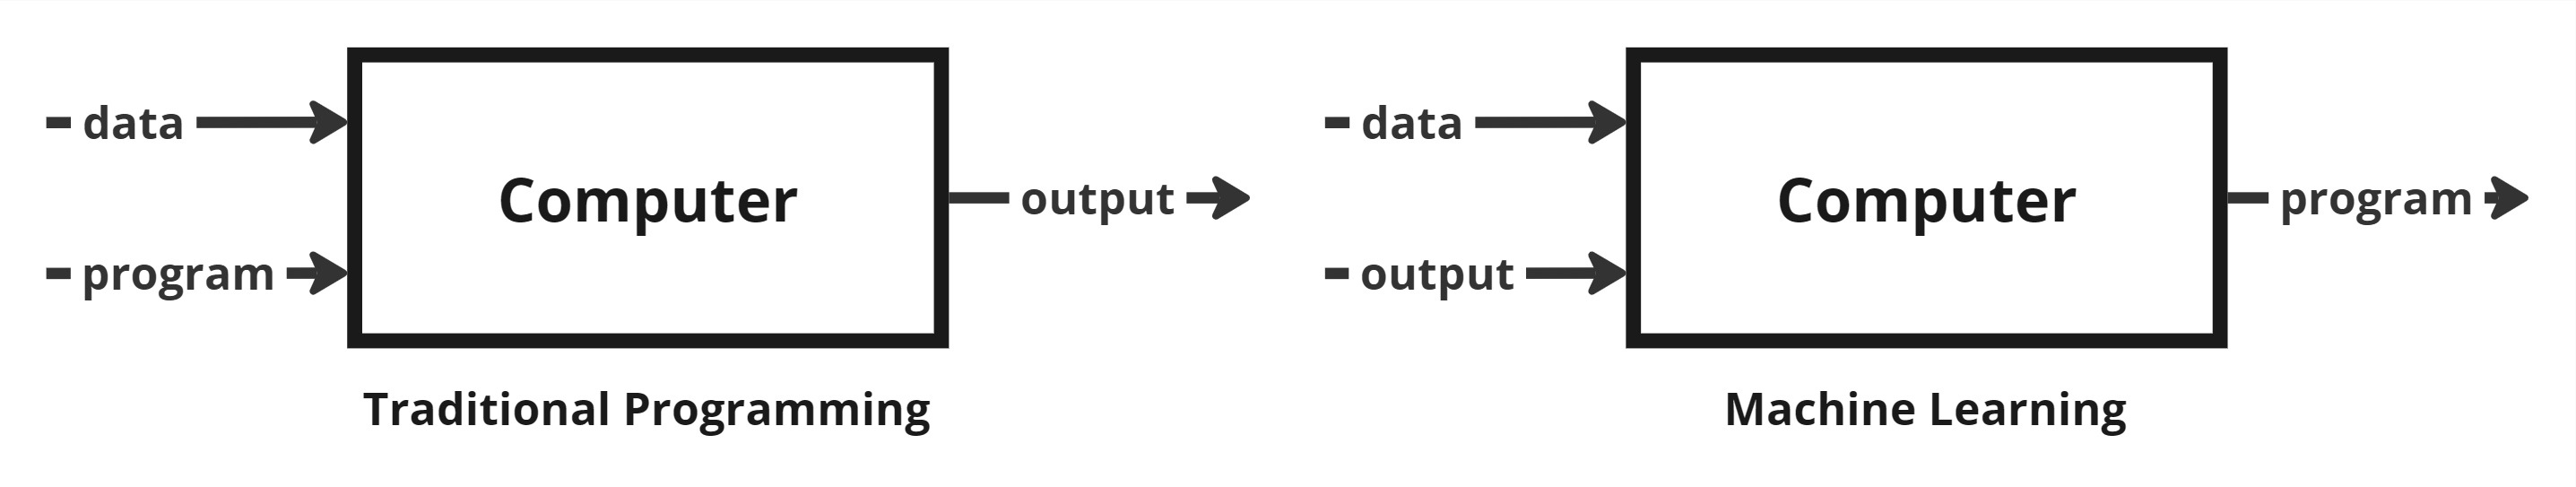
\includegraphics[width=0.5\linewidth]{images/Machine Learning Paradigm.jpg}
    \caption{Machine Learning Paradigm}
    \label{fig:machine_learning_paradigm}
\end{figure}

\noindent There are three main types of machine learning agents:
\begin{enumerate}
    \item \textbf{Supervised Learning}: given a set of desired outputs $y_1, ..., y_n$, the agent learns to produce the correct output for a new set of unseen values. The outputs from which the agent learns are called \textbf{labels}.
    \item \textbf{Unsupervised Learning}: the agent exploits patterns and regularities in the experience collected (encoded as a dataset $D = x_1, ..., x_n$). In this case there's no desired output to predict and no feedback. The most common unsupervised learning task is called \textbf{clustering}, which detects useful clusters from the input example.
    \item \textbf{Reinforcement Learning}: the agent performs actions $a_1, ..., a_n$ that effect the environment and receives a reward $r$. The agent learns to maximize its long term reward. To do so, it needs:
    \begin{itemize}
        \item decision process.
        \item reward system.
        \item long term expectations.
        \item learning sequence of actions.
    \end{itemize}
    This type of machine learning algorithms are the closest one to the ones studied so far.
\end{enumerate}

The most effective of these types of machine learning agents are the \textit{reinforcement learning} ones, as they can learn from their own actions and experience, by considering their ultimate success or failure. In reinforcement learning, the agent perceives, at time $t_0$, the environment to be in state $s_{t_0}$ and decides to perform an action $a_{t_0}$. As a result, in the next time step $t_0+1$, the environment changes to state $s_{t_0+1}$ and the agent receives a reward $r_{t_0+1}$. 

The goal of the agent is to \textit{maximize the total amount of reward received} by computing an action-value function that maps state-action pairs to expected payoffs:
    $$Q(s_t, a_t) \to \textnormal{payoff}$$
or a state-value function mapping to expected payoffs:
    $$V(s_t) \to \textnormal{payoff}$$

If we know function $Q$, the problem is solved. The point is that reinforcement learning assumes that $Q$ is represented as a table, but in real world problems the number of possible inputs can be too large to compute, so we must find a way to approximate it. The problem is non-trivial.    

\subsection{Action Selection \& Policy}
At each time step, the agent must decide what action to take in step $t=t_0$ based an its current evaluation of the expected payoff in $s_t$ using a \textbf{policy function}. At any given point in time, the policy function $\pi(s_t)$ selects what action the agent should perform based on its payoff evaluation.

When the correct action to take is not immediately obvious, an agent may need to consider a sequence of actions that lead to a goal state or, for short, to plan ahead of time. Such an agent is called \textbf{problem-solving agent} and the computational process is called \textbf{search}. The policy can be of two main types:
\begin{enumerate}
    \item \textbf{deterministic}: the policy function can be modeled as $\pi: S \to A$. This type of policy can be conveniently represented as a table.
    \item \textbf{stochastic}: the policy function maps each state to a probability distribution over the actions. The function can be modeled as $\pi: S\times A\to R$, which returns the probability of selecting the action $a$ in state $s$. Since $\pi(s, a)$ is a probability distribution, it returns a value between 0 and 1, and the sum over all the actions is always 1.
\end{enumerate}

\noindent
In order to obtain the maximum amount of reward, the agent must prefer actions that has tried in the past and found to lead to a high payoff. However, to discover those actions, it has to try actions that has never selected before. So the agent needs to find a trade-off between exploration of new actions and the exploitation of promising actions. This is called \textbf{exploration-exploitation dilemma}, which can be modeled in:
\begin{enumerate}
    \item Greedy policies: for each state the policy deterministically selects an action with maximal value.
    \item $\varepsilon$-Greedy policies: with probability $\varepsilon$ the policy selects a random action and with probability $1-\varepsilon$ selects an action promising the highest payoff.
\end{enumerate}

\subsection{Environment}
The environment must satisfy the Markov property: the next state $s_{t+1}$ and reward $r_{t+1}$ only depend on the current state $s_t$ and the taken action $a_t$. Thus, the environment can be modeled as \textbf{Markov Decision Process} (MDP for short), which has a one-step dynamic described by the probability distribution $p(s_{t+1}, r_{t+1}|s_t, a_t)$ such that:
$$p:S \times R \times S \times A \to [0, 1]$$
$$\sum_{s'\in S}\sum_{r\in R} p(s', r| s, a) = 1 \;\; \forall s \in S, \forall a \in A(s)$$

\subsection{Expected Payoff}
In reinforcement learning, the agent has to maximize the reward it receives in the long run, such that
$$G_t = r_{t+1} + r_{t+2} + ... + r_{t+k} + ... \to \infty$$
As shown, the problem with the $G$ function is that it tends to add up to infinity. To provide an upper bound to the payoff, we introduce a discount factor $\gamma$, such that $0 < \gamma < 1$ for future rewards, obtaining the following function
$$G_t = r_{t+1} + \gamma \cdot r_{t+2} + \gamma^2 \cdot r_{t+3} + ... + \gamma^{k-1} r_{t+k} + ... < \infty $$

Thus, the expected reward to maximize would be defined as
$$\mathbb{E}[G_t] = \mathbb{E}\left[\sum_{k=0}^{\infty}\gamma^k r_{t+k+1}\right] \le R_{max}\frac{1}{1-\gamma}$$

\subsection{Value Function}
The action-value function $Q(s_t, a_t)$ estimates the expected future payoff when performing action $a_t$ in state $s_t$. The state-value function $V(s_t)$ estimates the expected future payoff starting from state $s_t$. Both functions can be decomposed as the sum of the immediate reward received $r_{t+1}$ and the future rewards, so they become:
$$V(s) = \mathbb{E}[r_{t+1}+\gamma V(s_{t+1}|_{s_t=s})]$$
$$Q(s,a) = \mathbb{E}[r_{t+1}+\gamma  V(s_{t+1}|_{s_t =s,\; a_t = a})]$$

An agent based on the $Q$ function is called a \textbf{Q-learning agent}. At the beginning, the table $Q(\cdot, \cdot)$ is filled with random values, but at any time $t$ the table is filled with the values provided by the following formula:
$$Q(s_t, a_t) = Q(s_t, a_t) + \beta(r_{t+1} + \gamma  \max_{a\in A}Q(s_{t+1}, a) - Q(s_t, a_t)) $$

\clearpage
\noindent
where:
\begin{itemize}
    \item $\gamma$ is the discount factor;
    \item $\beta$ is the learning rate;
    \item $\pi(s_t, a_t)$ is the action selection strategy: the $\varepsilon$-greedy policy is commonly used during learning, but sufficient exploration must guarantee to tackle the exploration-exploitation dilemma.
\end{itemize}

Tabular representation in q-learning agents is mostly infeasible in practice so approximators must be used. Reinforcement learning computes an unknown value function while also trying to approximate it. Approximators work on intermediate estimates while providing information for the learning agent.

\clearpage
\section{Logical Agents}
A logical agent, also known as a \textbf{knowledge-based agent}, uses a process of reasoning over an internal representation of knowledge to decide what actions to take. The basic idea behind logical agents is that the states are represented in a structural way by a set of objects and relations between them. 

\subsection{Knowledge-Based Agents}
The central component of a logical agent is the \textbf{knowledge base}, or \textbf{KB}, which is a set of sentences expressed in a language called \textbf{knowledge representation language}. Each sentence expresses some assertion about the world with which the agent interacts. When a sentence is taken as being given without being derived from other sentences, we call it an \textbf{axiom}.

There must be a way to add new sentences to the knowledge base and a way to query what the agent knows. The standard names for these operations are \code{TELL} and \code{ASK}, and may involve some sort of \textbf{inference} (reasoning), that is deriving new sentences from old ones already known.

Like every other agent, the knowledge-based ones take a percept as input and returns an action as output, but it also maintains a knowledge base, which may initially be filled with some background knowledge. Ideally, logical agents could determine the next action to perform through reasoning, although in practice agents combine search and reasoning techniques.

\begin{figure}[h]
    \centering
    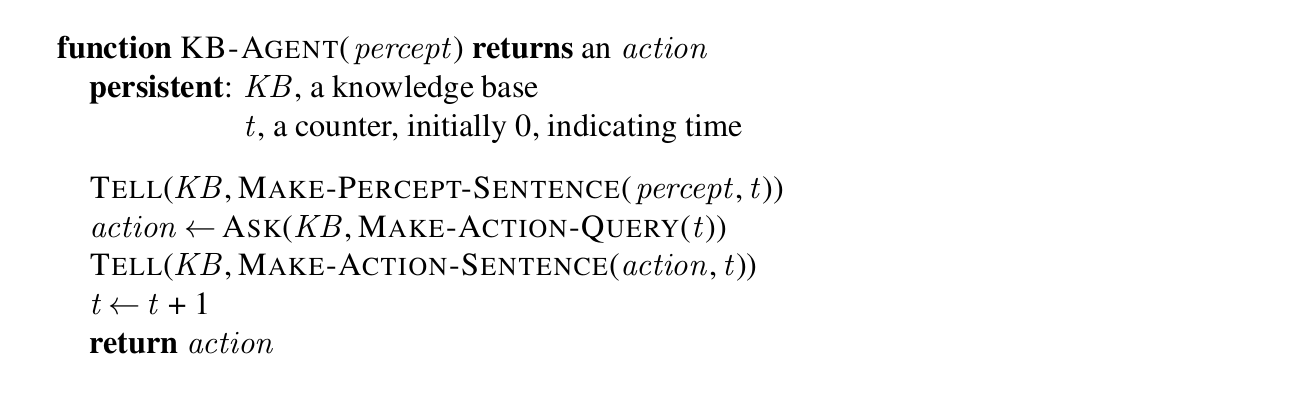
\includegraphics[width=1\linewidth]{algorithms/KB Agent.png}
    \label{fig:kb_agent_algorithm}
\end{figure}

\noindent
Each time the agent's program is called, it does three things:
\begin{enumerate}
    \item tells the knowledge base what has perceived of the world.
    \item asks the knowledge base what action should it perform. In the process of answering to this question, the agent may do extensive reasoning about the current state of the world and how it could change after performing some sequence of actions.
    \item tells the knowledge base which action was chosen and returns the action so it can be executed by the actuators.
\end{enumerate}

The knowledge based agent is not an arbitrary program that calculates actions, but it is amenable to a description at the knowledge level, where we need to specify only what the agent knows and what its goals are in order to determine its behavior. This type of agent can be built by simply telling it what it need to know. There are two approaches used to populate the knowledge base:
\begin{enumerate}
    \item \textbf{Declarative}: the agent starts with an empty knowledge base and the designer tells it sentences one by one until the agent knows exactly how it should operate in the world.
    \item \textbf{Procedural}: the desired behaviors of the agent are directly encoded in its program.
\end{enumerate}
We can also provide a knowledge-based agent with mechanisms that allow it to learn from itself and the environment in which it operates.

In logical agents the knowledge base and the inference engine are independent from each other; this means that the code for the engine is general and works for every agent, while the knowledge base is domain specific. So, the advantages of this type of agent are multiple:
\begin{itemize}
    \item Agents are described according to what they know, not according to how they are implemented.
    \item Only a core of essential information is explicitly represented, while the rest of the needed information can be derived.
    \item A logical agent can answer any type of question given the available knowledge, so we are not bounded to the previous search-based ones.
\end{itemize}

\subsection{Logic}
As already said, the knowledge base consists of sentences. Every sentence is expressed according to the \textbf{syntax} of the representation language, which specifies all the sentences that are well formed. A logic must also define the \textbf{semantics}, also known as meaning, of these sentences. In standard logic, every sentence must be either true or false. The semantics defines the truth of the sentence with respect to a \textbf{model}, which is a mathematical abstraction that defines a truth value for every relevant sentence.  If a sentence $\alpha$ is true in a certain model $m$, we say that $m$ satisfies $\alpha$ or that $m$ is a model for $\alpha$. We use the notation $M(\alpha)$ to mean the set of all models of the sentence $\alpha$.

Logical reasoning involves the relation of logical \textbf{entailment} between sentences, which is the idea that a sentence follows logically from another sentence. In mathematical notation, we write that $\alpha\models\beta$ to say that sentence $\alpha$ entails sentence $\beta$. More formally: $\alpha\models\beta$ if and only if, in every model in which $\alpha$ is true, $\beta$ is also true. Mathematically this notion is expressed as:
$$\alpha \models \beta \;\; \text{\textit{if and only if}} \;\; M(\alpha) \subseteq M(\beta)$$
Note that if $\alpha \models \beta $ then $\alpha$ is a stronger assertion than $\beta$, as it rules out more possible models. The procedure of carrying out new sentences from the old ones is also called \textbf{logical inference} \footnote{We can think of the set of all consequences of \textit{KB} as a \textit{haystack} and of $\alpha$ as a \textit{needle}. Entailment is the needle being in the haystack; inference is like finding it.}. \textbf{Model checking} is the procedure of enumerating all possible models to check that a sentence $\alpha$ is true in all models in which \textit{KB} is also true, that is $M(KB)\subseteq M(\alpha)$


If an inference algorithm $i$ can derive a sentence $\alpha$ from the \textit{KB}, we write that
    $$KB \vdash_i\alpha$$
which means that "$\alpha$ is derived from \textit{KB} by \textit{i}".

An inference algorithm that derives only entailed sentences is called \textbf{sound} or \textbf{truth-preserving}. This property is highly desirable as unsound algorithms make things up as they proceed. 
Another highly desirable property of inference algorithms is \textbf{completeness}, which means that it can derive any sentence that is entailed.

\textit{If KB is true in the real world, then any sentence $\alpha$ derived from KB by a sound inference procedure is also true in the real world}. The correspondence between world and representation is illustrated in figure \ref{fig:representation_v_real_world}.

\begin{figure}[h]
    \centering
    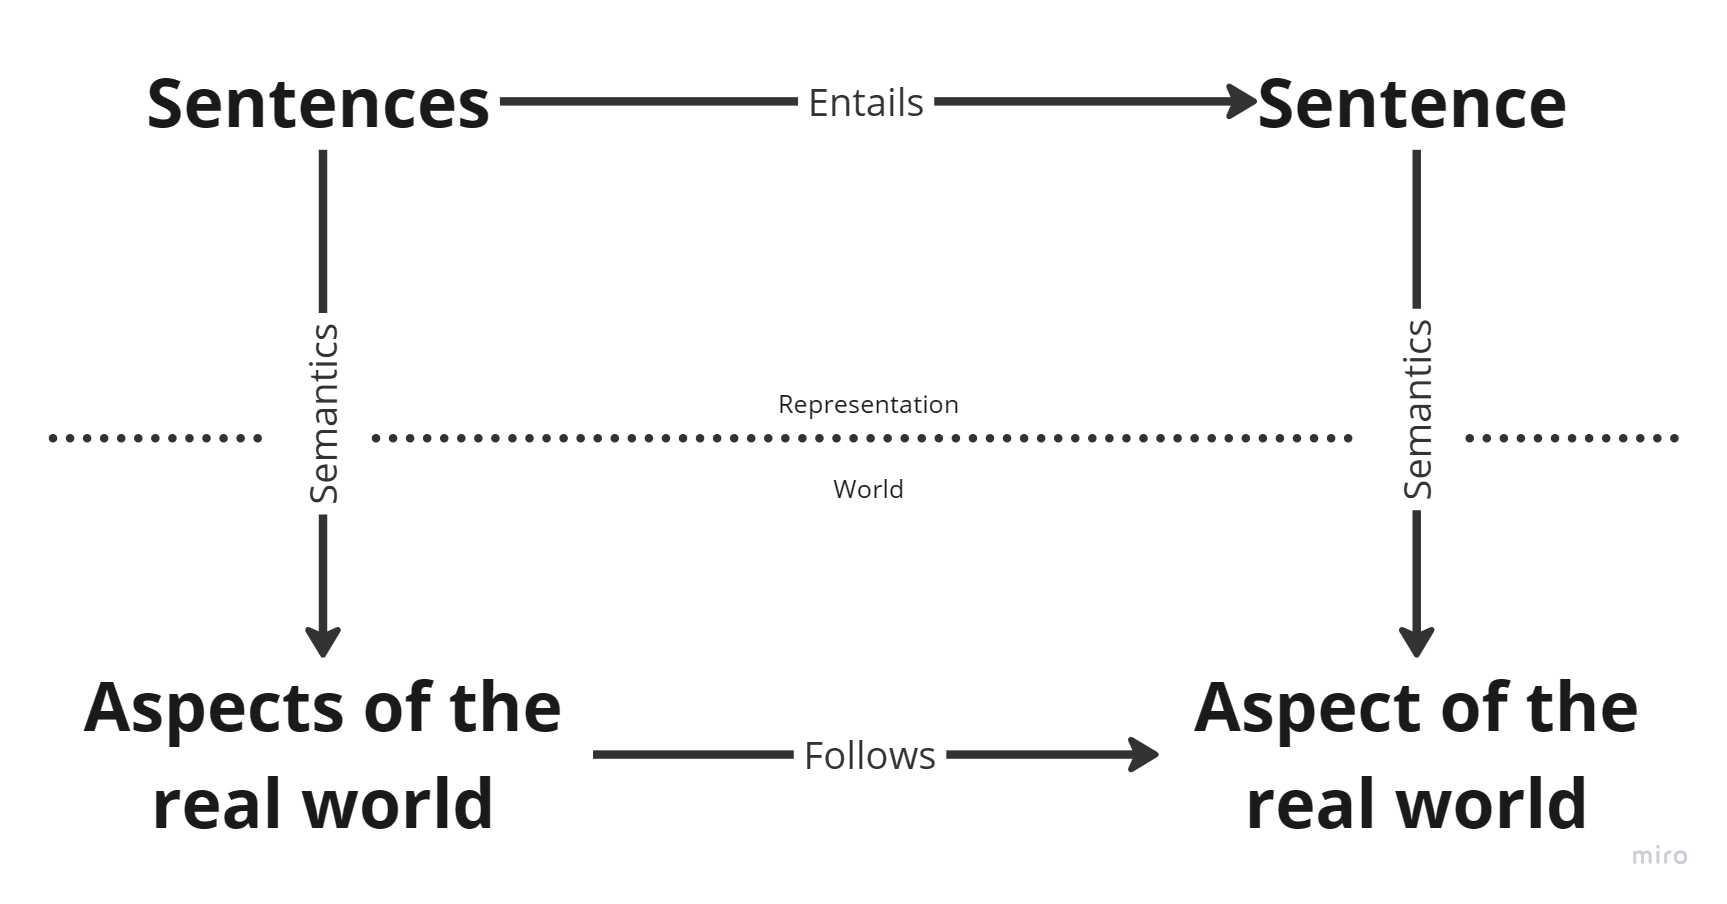
\includegraphics[width=0.5\linewidth]{images/Representation and Real World.png}
    \caption{Sentences are physical configurations of the agent, and reasoning is a process of constructing new physical configurations from older ones. Logical reasoning should ensure that the new configurations represent aspects of the world that actually follow from the aspects that the old configurations represent.}
    \label{fig:representation_v_real_world}
\end{figure}

\subsubsection{Propositional Logic}
The simplest type of logic is \textbf{propositional logic}. The syntax of propositional logic defines the allowable sentences. \textbf{Atomic sentences} consist of a single \textbf{proposition symbol}, which can be either true or false. There are two proposition symbols with fixed meanings: \textit{true} is the always true proposition and \textit{false} is the always false proposition. Complex sentences are constructed from simpler ones using parentheses and operators called \textbf{logical connectives}. There are five common connectives:
\begin{itemize}
    \item [$\neg$] is called the \textbf{negation}. A \textbf{literal} is either an atomic sentence (a positive literal) or a negated atomic sentence (a negative literal).
    \item [$\land$] is called \textbf{conjunction}. Its parts are \textbf{conjuncts}.
    \item [$\lor$] is called \textbf{disjunction}. Its parts are \textbf{disjuncts}.
    \item [$\Rightarrow$] is called \textbf{implication}. The first part is called \textbf{premise} or \textbf{antecedent}, while the second one is called \textbf{conclusion} or \textbf{consequent}.
    \item [$\Leftrightarrow$] is called \textbf{bi-conditional}.
\end{itemize}

The semantics of propositional logic defines the rules for determining the truth of a sentence with respect to a particular model: in simpler words, the model defines the truth value for every proposition symbol. The semantics for propositional logic must specify how to compute the truth value of any sentence, given a model, which is done recursively. The rules for atomic sentences are simple:
\begin{itemize}
    \item \textit{true} is true in every model and \textit{false} is false in every model.
    \item The truth value of every other proposition symbol must be specified directly in the model.
\end{itemize}

\noindent
The rules for complex sentences are, obviously, more complex:
\begin{itemize}
    \item $\neg P$ is true iff $P$ is false in $m$.
    \item $P \land Q$ is true iff both $P$ and $Q$ are both true in $m$.
    \item $P\lor Q$ is true iff either $P$ or $Q$ is true in $m$.
    \item $P\Rightarrow Q$ is true unless $P$ is true and $Q$ is false in $m$.
    \item $P \Leftrightarrow Q$ is true iff $P$ and $Q$ are both true or both false in $m$.
\end{itemize}

\noindent
The rules can also be expressed using truth tables that specify the truth value of a complex sentence for each possible assignment of truth values to its components, as follows:

\begin{table}[h]
    \centering
    \begin{tabular}{c|c||c|c|c|c|c}
        $P$ & $Q$ & $\neg P$ & $P \land Q$ & $P\lor Q$ & $P\Rightarrow Q$ & $P \Leftrightarrow Q$ \\ \hline\hline
        0 & 0 & 1 & 0 & 0 & 1 & 1 \\ \hline
        0 & 1 & 1 & 0 & 1 & 1 & 0 \\ \hline
        1 & 0 & 0 & 0 & 1 & 0 & 0 \\ \hline
        1 & 1 & 0 & 1 & 1 & 1 & 1
    \end{tabular}
\end{table}

Every complex sentence can be represented using a tree like structure, where every leaf is a simple sentence and every other node is a composition of those sentences through logical connectives.

The advantage of propositional logic is that allows \textbf{partial}, \textbf{disjunctive} and \textbf{negated} information, unlike most data structures and databases. Also, it is \textbf{compositional}, which means that the meaning of a complex sentences is derived from simpler ones. Moreover, the meaning in propositional logic is context independent, unlike natural language, where the meaning of a sentence may vary based on the context. The only problem with propositional logic is that it has limited expressive power, which makes it harder to express difficult problems.

\subsubsection{Inference Proof}
Our goal is to decide whether $KB \models \alpha$ for some sentence $\alpha$. The first algorithm we can use to reach our goal is \textbf{model-checking} which, as said before, enumerates all the models and checks that $\alpha$ is true in every model in which \textit{KB} is true. This algorithm is sound because it implements directly the definition of entailment, and it is also complete because it works for any \textit{KB} and $\alpha$ and always terminates, because there are a finite number of models to examine.

Another way to reach our goal is by \textbf{theorem proving}, which applies rules of inference directly to the sentences in our KB to construct a proof of the desired sentence without consulting models. In order to examine this approach we need some basic concepts:
\begin{itemize}
    \item \textbf{Logical equivalence}: two sentences $\alpha$ and $\beta$ are logically equivalent if they are true in the same set of models. We write 
        $$\alpha\equiv\beta \;\text{if and only if}\; \alpha\models\beta \;\text{and}\; \beta\models\alpha.$$
    
    \item \textbf{Validity}: a sentence is valid if it is true in \underline{all} models. Valid sentences are also known as \textbf{tautologies}. Because the sentence \textit{true} is true in every model, every valid sentence is logically equivalent to \textit{true}. From this, we can derive the \textbf{deduction theorem}:
        $$\text{For any sentence}\; \alpha \;\text{and}\; \beta, \alpha\models\beta \;\text{if and only if}\; (\alpha\Rightarrow\beta) \;\text{is valid}.$$
    Hence we can decide if $\alpha\models\beta$ by proving that $(\alpha\Rightarrow\beta)\equiv true$.
    
    \item \textbf{Satisfiability}: a sentence is satisfiable if it is true in \underline{\textbf{some}} model.
\end{itemize}

\noindent Validity and satisfiability are connected: $\alpha$ is valid iff $\neg\alpha$ is unsatisfiable, and $\alpha$ is satisfiable iff $\neg\alpha$ is not valid. We obtain the following result:
    $$\alpha\models\beta \;\text{if and only if the sentence}\; (\alpha\land\neg\beta) \;\text{is unsatisfiable}.$$
Which is called proof by \textbf{refutation} or proof by \textbf{contradiction}.

\subsubsection{First Order Logic - FOL}
Propositional Logic is very limited in what it can express: we can adopt the foundation of propositional logic and build a much more expressive logic, based on \textbf{objects}, \textbf{relations} and \textbf{functions}. This new type of logic is called \textbf{First Order Logic} (or \textbf{FOL}).

The models of a logical language are the formal structures that constitute the possible worlds under consideration. Each model links the vocabulary of the logical sentences to elements of the possible world, so that the truth of any sentence can be determined. In propositional logic, the models simply link proposition symbols to predefined truth tables, while the models in first order logic are much more interesting as they contain objects.
The \textbf{domain} of a model is the set of objects, called \textbf{domain objects}, it contains. The domain is required to be non-empty. The objects in the model may be related in some ways: a relation is just the set of tuples of objects that are related. Models can contain \textbf{binary} relationships, which relate a pair of objects, or unary relations called \textbf{properties}. Certain kind of relationships are best considered as functions, in that a given object must be related to exactly one object in this way.

The basic syntactic elements of FOL are symbols that stand for objects, relations and functions. There are three kind of symbols:
\begin{enumerate}
    \item \textbf{Constant symbols}, which stand for objects.
    \item \textbf{Predicate symbols}, which stand for relations.
    \item \textbf{Function symbols}, which stand for functions.
\end{enumerate}
\noindent Each predicate and function symbol comes with an \textbf{arity}, that describes the number of arguments it receives.

Every model must provide some information to determine if any given sentence is true or false. Thus, in addition, every model includes an interpretation that specifies exactly which objects, relations and functions are referred to by the constant, predicate and function symbols.

A \textbf{term} is a logical expression that refers to an object. Constant symbols are terms, but it's not always convenient to have distinct symbols to name every object, in the same way we do not give a specific name to every object in reality. Considering a term $f(t_1, ..., t_n)$, the symbol \textit{f} refers to some function in the model (call it \textit{F}), the argument terms refer to objects in the domain (call them $d_1, ...,d_n$) and the term as a whole refers to the object that is the value of the function \textit{F} applied to the terms $d_1, ...,d_n$.

Now we can combine terms and symbols to make \textbf{atomic sentences} that state facts. An atomic sentence, or atom for short, is formed from a predicate symbol optionally followed by a parenthesized list of terms. \textit{An atomic sentence is true in a given model if the relation referred to by the predicate symbol holds among the objects referred to by the arguments}. We can use logical connectives to construct more complex sentences.

Once we have a logic that allows objects, we can use \textbf{quantifiers} to express properties of entire collections of objects, instead of enumerating them one by one. There are two types of quantifiers:
\begin{itemize}
    \item [$\forall$] - \textbf{universal quantifier}. The sentence $\forall x P$, where \textit{P} is any logical sentence, says that \textit{P} is true for every object \textit{x}. By asserting the universally quantified sentence, which is equivalent to asserting a whole list of individual implications, we end up asserting the conclusion of the rule just for those objects for which the premise is true and saying nothing about those objects for which the premise is false. Thus, the truth table definition of $\Rightarrow$ turns to be perfect for writing general rules for universal quantifiers.
    \item [$\exists$] - \textbf{existential quantifiers}. The sentence $\exists x P$ says that \textit{P} is true for at least one object \textit{x}. Just like $\Rightarrow$ is the natural connective to use with the universal quantifier, $\land$ is the natural connective to use with $\exists$.
\end{itemize}

Consecutive quantifiers of the same type can be written as one quantifier with several variables:
$$\forall x_1 ... \forall x_n \equiv \forall x_1,...,x_n \;\;\text{and}\;\; \exists x_1, ..., \exists x_n \equiv \exists x_1,...,x_n$$
In all other cases, the order in which the quantifiers appear is very important, as it can lead to very different statements.

The two quantifiers are actually intimately connected with each other through negation:
\begin{align*}
    \forall x P & \equiv \neg\exists x \neg P \\
    \exists x P & \equiv \neg\forall x \neg P \\
    \neg\forall x P & \equiv \exists x \neg P \\
    \neg\exists x P & \equiv \forall x \neg P \\
\end{align*}

One last symbol in FOL is the \textbf{equality symbol}, which signifies that two terms refer to the same object. Also, the notation $x\neq y$ is used as an abbreviation for $\neg(x=y)$.

\subsection{Inference for Propositional Logic - Model Checking}
As already said, the goal of inference procedures is to demonstrate that a sentence $\alpha$ entails another sentence $\beta$. There are two main methods used:
\begin{enumerate}
    \item \textbf{Model-checking}: an algorithm $A$ checks if for every model in which $\alpha$ is true, $\beta$ is also true.
    \item \textbf{Theorem-proving}: an algorithm $A$ builds a demonstration (or a proof) that leads from $\alpha$ to $\beta$ ($\alpha \vdash_A \beta$). The algorithm must be:
    \begin{itemize}
        \item \textbf{Sound}: everything the algorithm claims to prove is entailed.
            $$\alpha \vdash_A\beta\Rightarrow\alpha\models\beta$$
        \item \textbf{Complete}: everything the algorithm entails can be proved. 
            $$\alpha\models\beta\Rightarrow\alpha\vdash_A\beta$$
    \end{itemize}        
\end{enumerate}

Certain applications of propositional logic require the agent to establish whether a sentence $\alpha$ is or is not satisfiable, which means whether there is an assignment of truth values to the symbol $\alpha$ that makes it true. The problem of establishing the satisfiability of a set of propositional sentences is known as \textbf{SAT}. The problem of establishing propositional entailment can be reduced to an SAT problem. A solution of SAT is given by reasoning using truth tables, but this is a rather inefficient method. A more efficient one is provided by the DPLL algorithm.

\subsubsection{Reasoning by Truth Tables}
One first approach we can take to solve the problem is to reason with truth tables. This approach is a form of semantic reasoning, as it directly exploits the definition of entailment: $\alpha\models\beta$ holds when $\beta$ is true in every model that makes $\alpha$ true. In propositional logic, a model is the assignment of truth values to every propositional symbol that appears in $\alpha$, $\beta$ or both. The problem is that with \textit{n} symbols we have $2^n$ different possible models, which corresponds to a row of the truth table. The algorithm computes for every model (each row) the truth values of $\alpha$ and $\beta$ by recursively computing the truth values of all sub-sentences of $\alpha$ and $\beta$. At last, we have that $\alpha\models\beta$ if and only if every row that assign 1 to $\alpha$, also assigns 1 to $\beta$. The same logic can be used to demonstrate $KB\models\beta$, where $KB=\alpha_1\land\alpha_2\land...\land\alpha_n$.

This process is sound and complete, and it is also decidable as it always terminates. However the described algorithm is very inefficient when many propositional symbols are involved, because it has to compute a table of size $2^n\cdot M$, where \textit{n} is the number of propositional symbols and \textit{M} is the number of sub-sentences that appear in the premises and the conclusion. This process is also very unnatural for humans, making it problematic in those applications in which the artificial agent must be able to justify the conclusions of its reasoning process.

\subsubsection{DPLL Algorithm}
The DPLL Algorithm establishes whether or not a sentence $\alpha$ is satisfiable. It takes as input a sentence in \textbf{Conjunctive Normal Form} and incrementally tries to build a model of $\alpha$ from an empty assignment: if a model is built, $\alpha$ is satisfiable, otherwise, if the algorithm ends without being able to build a model, $\alpha$ is not satisfiable. Essentially, this algorithm is a recursive, depth-first enumeration of all possible models for a sentence $\alpha$ in CNF.

A CNF represents a sentence as a conjunction of clauses, where every clause is a disjunction of literals, which are either a propositional symbol or the negation of a symbol. Every sentence of propositional logic can be transformed in an equivalent sentence in conjunctive normal form. A CNF sentence is often considered as a set of clauses in logical conjunction, which are in turn considered as sets of literal in logical disjunction. 

Every sentence of propositional logic can be transformed into a CNF clause, following these steps:
\begin{enumerate}
    \item Eliminate $\Leftrightarrow$: $\alpha \Leftrightarrow \beta \equiv (\alpha \Rightarrow \beta) \land (\beta \Rightarrow \alpha)$.
    \item Eliminate $\Rightarrow$: $\alpha \Rightarrow \beta \equiv \neg \alpha \lor \beta$.
    \item CNF requires $\neg$ to appear only in literals, so we move the negation inwards by applying the De Morgan rules (see appendix \ref{appendix:Logic}).
\end{enumerate}

A unit clause is a clause with only one literal. Two literals are complementary if they refer to the same propositional symbol but one is the negation of the other, like \textit{A} and $\neg A$. In order to transform a PL sentence in the conjunctive normal form we use the De Morgan rules.

\noindent 
The DPLL algorithm is essentially a depth first search with back-tracking over logical models, with the following extra steps:
\begin{enumerate}
    \item \textbf{Early termination}: the algorithm detects whether the sentence must be true or false even with a partially completed model. A clause is true if \underline{any} of its literals are true, even if the other literals do not yet have truth values. Early termination avoids examination of entire sub-trees in the search space.
    \item \textbf{Pure symbol heuristic}: a pure symbol is a symbol that always appears with the same "sign" in all clauses. If a sentence has a model, then it has a model with the pure symbol assigned so as to make their literals true, because doing so can never make a clause false. In determining the purity of a symbol, the algorithm can ignore clauses that are already known to be true in the model constructed so far.
    \item \textbf{Unit clauses heuristic}: a unit clause, in the context of DPLL, are clauses in which all literal but one are already assigned false by the model (so the truth depends on the unassigned literal). The unit clause heuristic assigns all such symbols before branching on the reminder. One important consequence of this heuristic is that any attempt to prove a literal that is already in the knowledge base will succeed immediately. Also, assigning one unit clause can create another unit clause, producing a cascade of forced assignments called unit propagation.  
\end{enumerate}

\begin{figure}[h]
    \centering
    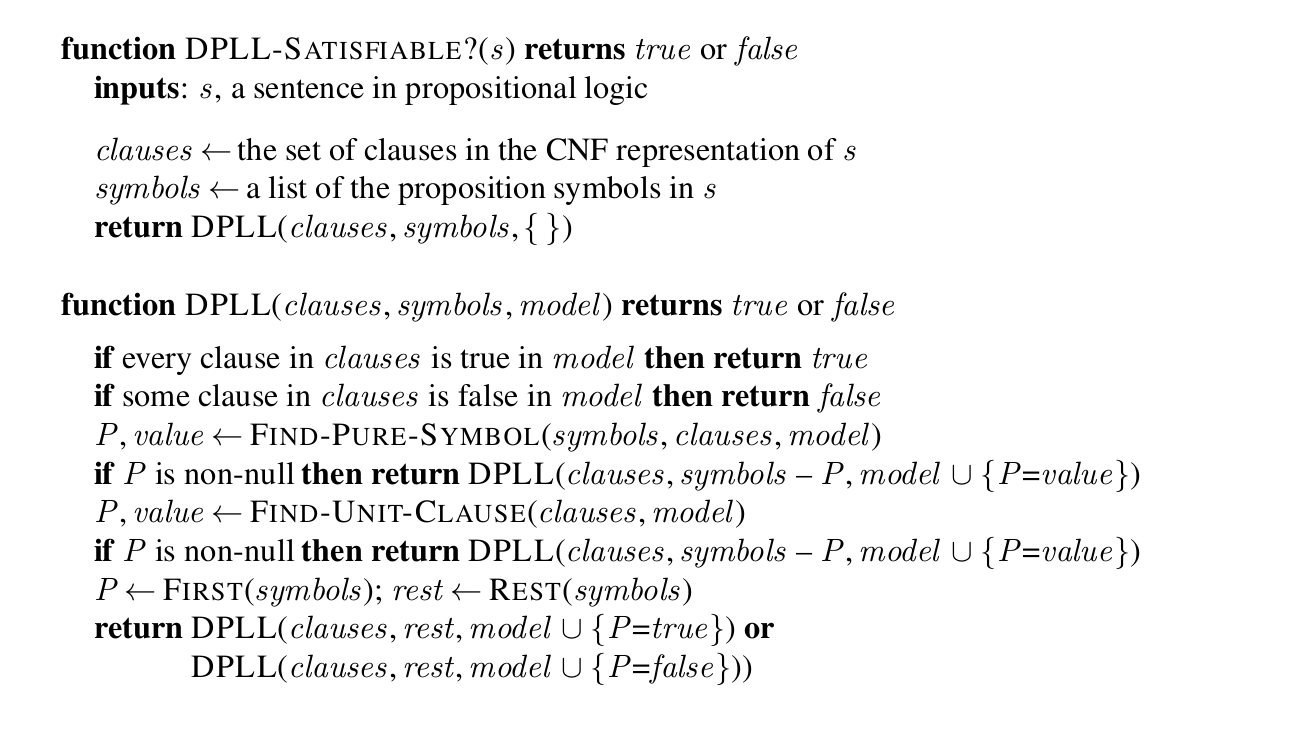
\includegraphics[width=1\linewidth]{algorithms/DPLL.png}
    \label{fig:dpll_algorithm}
\end{figure}

As already said, the problem of establishing propositional entailment can be reduced to a SAT problem, because $\alpha \models \beta$ holds if and only if, equivalently:
\begin{itemize}
    \item every model that satisfies $\alpha$ also satisfies $\beta$.
    \item no model satisfies both $\alpha$ and $\neg \beta$.
    \item $\alpha \land \neg \beta$ is unsatisfiable.
\end{itemize}

\noindent 
In this case the proof of entailment works by refutation: to prove that $\alpha \models \beta$ it proves that $\alpha \land \neg \beta$ is unsatisfiable, so it builds a refutation for $\alpha \land \neg \beta$ by showing the impossibility to find a model.  

A naive implementation of the DPLL algorithm can solve a sentence with approximately 100 variables before being impractical. Some improvements we can make are the following:
\begin{itemize}
    \item Variable and value ordering (from the CSP).
    \item Divide and Conquer.
    \item Caching unsolvable sub-cases as extra clauses to avoid redoing them.
    \item Smart Indexing and incremental recomputation tricks so that every step of the DPLL algorithm is efficient (with a time complexity of $O(1)$).
\end{itemize}

\subsection{Inference for Propositional Logic - Theorem Proving}
As already said in the previous section, an inference procedure aims to demonstrate that $\alpha \models \beta$ by using an algorithm \textit{A}, that uses propositional logic. 

Inference rules can be applied to derive a proof, which is a chain of conclusions that leads to the desired goal. The best-known rule is the \textbf{Modus Ponens} written as follows:
$$\frac{\alpha \Rightarrow \beta, \;\; \alpha}{\beta}$$
This notation means that, whenever any sentence of the form of $\alpha \Rightarrow \beta$ and $\alpha$ are given, the sentence $\beta$ can be inferred.

Another useful inference rule is the \textbf{And-Elimination}, which says that from a conjunction any of the conjuncts can be inferred:
$$\frac{\alpha \land \beta}{\alpha}$$

Both rules are \textit{sound} and can be used in any sentence where they apply generating inference without the need for enumerating every possible model. 

There are three main algorithms used for theorem proving.

\subsubsection{Propositional Resolution}
Propositional resolution is an extremely powerful inference procedure for propositional logic, as it yields a complete inference algorithm when coupled with any complete search algorithm. Propositional resolution works by refutation on any set of sentences in conjunctive normal form. In practice, propositional resolution works by trying to find the empty clause ($\perp$) from the set of clauses contained in $KB \land \neg \alpha$. Resolution applies the resolution rule to all clauses, also to the ones derived by the previous applications of the resolution rule: given two clauses $C_1$ and $C_2$ containing respectively $\ell$ and $\ell^c$, then both clauses can be resolved into a new clause $C$ called \textbf{resolvent}, such that $C=(C_1 - \{\ell\})\cup(C_2-\{\ell^c\})$.

This is called the \textbf{unit resolution} inference rule:
$$\frac{\ell_1 \vee \cdots \vee \ell_k,\;\; m}{\ell_1\vee \cdots \ell_{i-1}\vee\ell_{i+1}\vee \cdots \vee \ell_k}$$
where $\ell$ is a literal and $\ell_i$ and \textit{m} are complementary literals. Thus, this rule takes a clause and a literal and produces a new clause. It can also be generalized to the full resolution rule:
$$\frac{\ell_1\vee\cdots\vee\ell_k,\;\; m_1\vee\cdots\vee m_n}{\ell_1\vee\cdots\vee\ell_{i-1}\vee\ell_{i+1}\vee\cdots\vee\ell_k\vee m_1 \vee m_{j-1}\vee m_{j+1}\vee\cdots\vee m_n}$$
where $\ell_i$ and $m_j$ are complementary literals. This rule takes two clauses and produces a new clause containing all the literals of the two original clauses except the two complementary literals. Using propositional resolution, it is possible to build a theorem prover that is sound and complete for propositional logic: in fact, resolution rule is sound, and the resolvent $C$ is satisfiable if and only if clause $C_1$ and $C_2$ are simultaneously satisfiable, but since resolvent is smaller than parent clauses, resolution stops at some point.

The resolution algorithm works by following these steps:
\begin{enumerate}
    \item $KB \land \neg \alpha$ is converted in CNF.
    \item The resolution rule is applied to the resulting clauses.
    \item Each pair that contains complementary literals is resolved to produce a new clause which is added to the set if it is not already present.
    \item The process continues until one of the following happens:
    \begin{itemize}
        \item There are no new clauses that can be added, in which case the \textit{KB} does not entail $\alpha$.
        \item Two clauses resolve to yield the \textit{empty} clause, in which case \textit{KB} entails $\alpha$.
    \end{itemize}
\end{enumerate}

The empty clause arises from resolving two contradictory unit clauses (such as $P \land \neg P$) and is equivalent to \textit{false} because a disjunction is true only if at least one of its disjuncts is true. Using propositional resolution, it is possible to build a theorem that is sound and complete for propositional logic.

\begin{figure}[h]
    \centering
    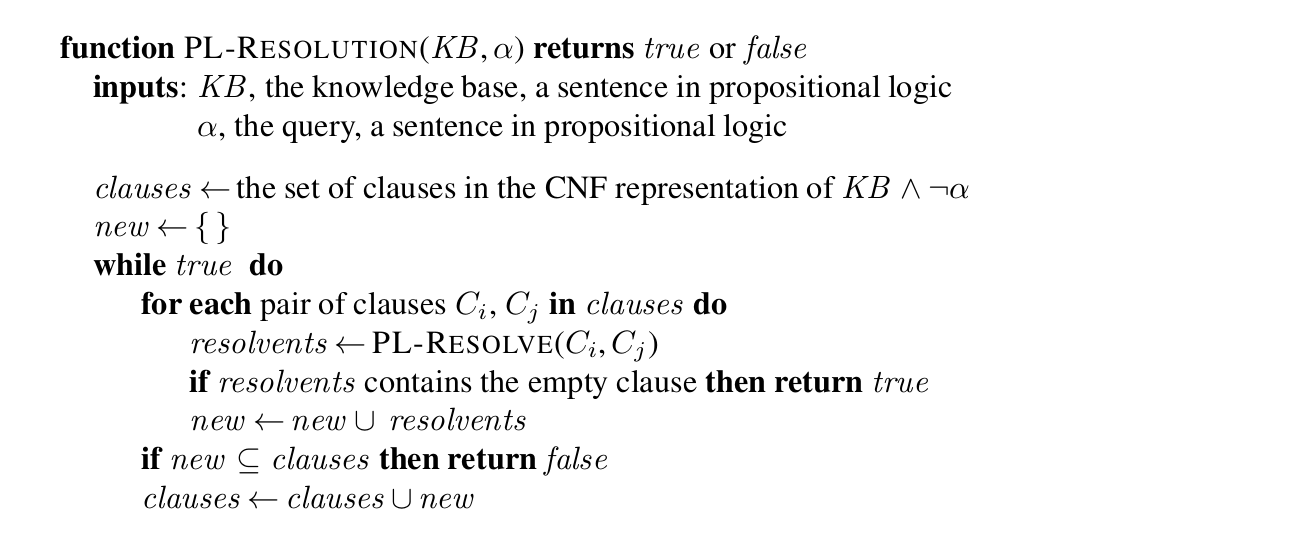
\includegraphics[width=1\linewidth]{algorithms/PL Resolution.png}
    \label{fig:PL_resolution}
\end{figure}

\noindent
There are different resolution strategies we can apply to reach our goal:
\begin{itemize}
    \item \textbf{Unit resolution}: at least one of the parent clauses is a unit clause; this strategy is incomplete in general, but complete for Horn clauses.
    \item \textbf{Input resolution}: at least one of the two parent clauses is a member of the initial set of clauses; this strategy is incomplete in general, but complete for Horn clauses.
    \item \textbf{Linear resolution}: generalization of the input resolution method in which at least one of the parents is either in the initial set of clauses or in an ancestor of the other parent; this strategy is complete.
    \item \textbf{Set of support resolution}: given a set of support \textit{S}, which is a subset of the initial clauses such that the clauses not in \textit{S} are satisfiable, every resolution involves a clause in \textit{S} (the resolvent is added to \textit{S}).
\end{itemize}

\subsubsection{Forward and Backward Chaining}
The completeness of resolution makes it a very effective inference method, but in many practical situations it is too powerful. Som real-world knowledge based problems contains sentences which satisfy some restriction on their form, which enables more efficient inference algorithms. One of such restrictions is the \textbf{definite clause}, which is a disjunction of literals of which \underline{exactly one} is positive. A slightly more general restriction is the \textbf{Horn clause}, which is a disjunction of literals of which \underline{at most one} is positive. Horn clauses represent rules, facts, goals or empty clauses.

Knowledge bases containing only definite clauses are interesting for three main reasons:
\begin{enumerate}
    \item Every definite clause can be written as an implication whose premise in a conjunction of positive literals and whose conclusion is a single positive literal.
    \item Inference with Horn clauses can be done through \textbf{forward-chaining} and \textbf{backward-chaining} algorithms.
    \item Deciding entailment with Horn clauses can be done in time that is linear in the size of the knowledge base.
\end{enumerate}

The forward chaining algorithm determines if a single proposition symbol \textit{q} (called query) is entailed by a knowledge base of definite clauses. It begins from known facts \footnote{
\textbf{facts} are sentences consisting of a single positive literal.
} in the knowledge base and, if all the premises of an implication are known, the its conclusion is added to the set of known facts. This process iterates until the query \textit{q} is added or until no further inferences can be made. Forward chaining is a sound and complete algorithm, as every inference is an application of the Modus Ponens and every entailed atomic sentence will be derived. Forward chaining is also said to be \textbf{data-driven reasoning}, that is reasoning in which the focus of the attention starts with the known data. It is a type of "unconscious" processing, which can derive everything that is entailed by the knowledge base, but sometimes does a lot of work which is irrelevant to the specific goal.

\begin{figure}[h]
    \centering
    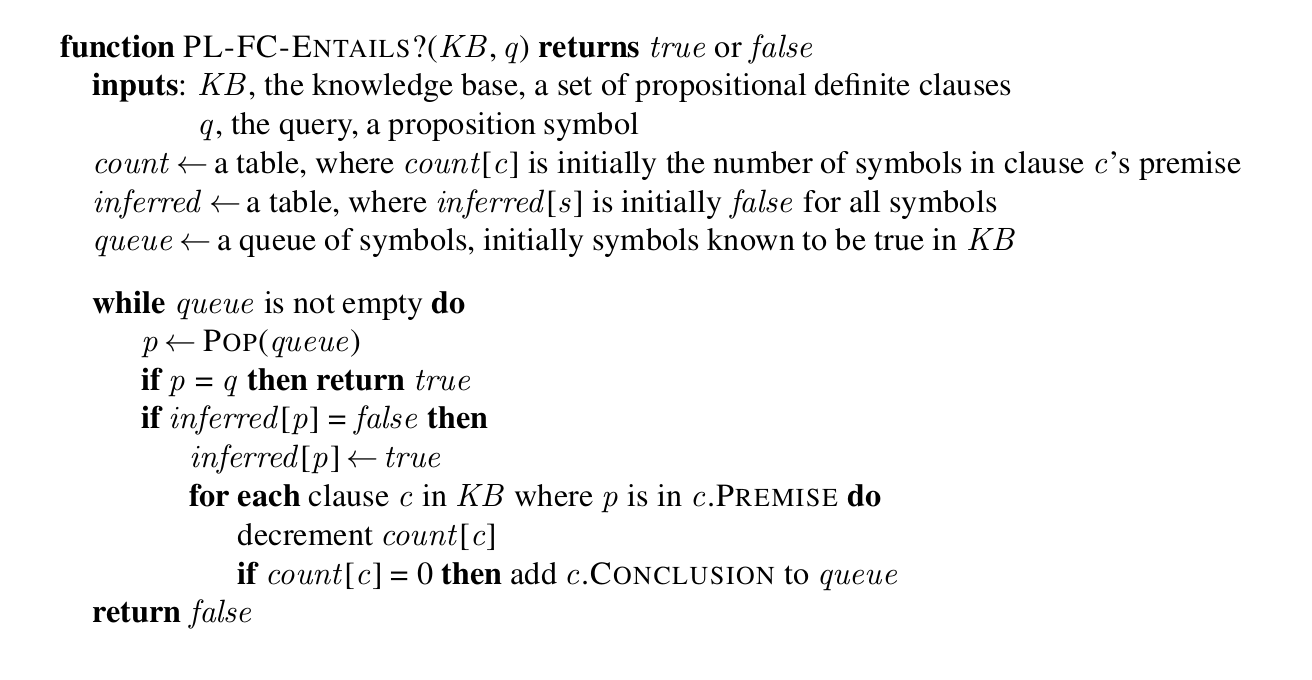
\includegraphics[width=1\linewidth]{algorithms/PL Resolution Forward Chaining .png}
    \label{fig:PL_resolution_with_forward_chaining}
\end{figure}

The backward chaining algorithm works backward from the query: if the query \textit{q} is known to be true, then no work is needed, otherwise, the algorithm finds those implications in the knowledge base whose conclusion is \textit{q}. If all the premises of one of the implications can be proved true, then also \textit{q} is true. Backward chaining is a form of \textbf{goal-directed reasoning}, which is appropriate for problem-solving. Backward chaining is sound and complete for knowledge bases composed of definite clauses, and has a complexity which can be much less than linear in the size of the knowledge base.

\clearpage
\section{Planning}
Classical planning is the task of finding a sequence of partially ordered actions to accomplish a goal in a \textit{discrete}, \textit{deterministic}, \textit{fully observable} and \textit{static} environment, using logical sentences to represent states, actions and goals. In other words, classical planning is some sort of specialization of generic search algorithms in which states, actions and goals are represented using logical sentences.

The knowledge for planning problems is represented by a \textbf{factored representation}, specifically:
\begin{enumerate}
    \item \textbf{STRIPS} (Stanford Research Institute Problem Solver) language: a simple, but rather expressive language based on a simplified version of first order logic (with no functions).
    \item \textbf{PDDL} (Planning Domain Definition Language): a family of languages (including STRIPS) used internationally.
\end{enumerate}

\subsection{PDDL}
PDDL uses \textbf{constants} to denote objects and \textbf{predicates} to represent properties of the objects and their relationship. A \textbf{state} is represented as a conjunction of \textit{positive ground atomic fluents}, in which positive means that negations are not allowed, ground means with no variables, fluent stands for aspects of the world that change over time and atomic means that there is a single predicate with optional constant arguments. No disjunctions are allowed and uncertainty is not represented.

The assumptions under which the state is represented are the following:
\begin{itemize}
    \item \textbf{Unique Name Assumption} (UNA): different constants \underline{always} denote different objects.
    \item \textbf{Domain Closure Assumption} (DCA): the environment includes only objects denoted by constants.
    \item \textbf{Closed World Assumption} (CWA): all literals that are not explicitly mentioned in the description of the state are considered to be false.
\end{itemize}

The \textbf{goals} are just conjunction of positive or negative literals (unlike STRIPS where only positive literals are allowed) also called \textit{sub-goals}, that may contain variables. A goal $g$ is satisfied in a state $s$ when all the sub-goals of $g$ are contained in the representation of the state $s$. Furthermore, a goal $g$ containing a variable is satisfied in state $s$ when there is at least one ground literal in $s$ that matches the variable in the goal.    

\textbf{Actions} consist of a name (denoting the action), a list of variables used, a \textbf{precondition}, that is a conjunction of literals in which variables are allowed, and an \textbf{effect}, formed by a \textit{delete list} (negative literals) and an \textit{add list} (positive literals). An action $a$ is \textbf{applicable} in state $s$ if all positive literals contained in the precondition of $a$ are also contained in the description of $s$, and all the negative literals in the precondition of $a$ are \underline{not} contained in $s$.
The application of action $a$ in $s$ generates a new state $s'$ by deleting from $s$ all the literals in the delete list (also called negative effects) and by adding the literals in the add list (also called positive effects) to the existing conditions in state $S$, such as
    
    $$s' = result(s,\;a) = (s - del(a)) \;\cup\; add(a)$$

An \textbf{action schema} is a family of actions parametrized by one variable $x$ (or more variables), that is instantiated to satisfy the preconditions in a state. Variables in delete list and in add list must also appear in preconditions (otherwise they are unbound) and in the signature of the action schema.

The solutions is called \textbf{plan}, which is an ordered sequence of actions that, starting from an initial state $s_0$, brings to a state $s_g$ that satisfies the goal $g$. As always, the optimal solution is the one with the minimum cost. 

The \textbf{frame problem}, for logical agents, is the problem of representing what remains unchanged after the application of a specific action. In PDDL the frame problem is avoided by two distinct mechanisms:
\begin{enumerate}
    \item The things that are changed by an action are only and exactly those specified in the effects (positive and negative literals)
    \item Anything that is not listed as an effect is left unchanged by the execution of the action
\end{enumerate}

\noindent
Therefore, there is no need to specify axioms.

\subsection{Forward Planning}
We can solve planning problems by applying any of the heuristic search algorithm previously analyzed: we search in the state space from the initial state $s_0$ to a state $s_g$ that satisfies the goal. The states in the search space are ground, where every fluent is either true or false, and the goal is a state where each fluent is positive. The applicable actions in a state, yielded by the $actions(s)$ function, are all the grounded instantiations of the action schemas. To determine the applicable actions, we unify the current state against the preconditions of each action schema. For each unification that successfully results in a substitution, we apply the substitution to the action schema to yield a ground action with no variables.

Any type of search strategy can be used to solve the search problem derived from forward planning. A heuristic function $h(s)$ can be defined by formulating a relaxed version of the problem that is easier to solve by substituting actual actions with actions without some or all preconditions. $h(s)$ is the cost of the optimal solution for the relaxed problem.

Forward planning can be very inefficient due to the huge branching factor as there are multiple actions that are applicable in a certain state, many of which are not relevant to reach the goal state.

\subsection{Backward Planning}
In backward search, also called \textbf{regression search}, we start at the goal state $s_g$\footnote{
    Let it be clear that in planning problems the goal $g$ is not a state, but a set of logic sentences. We say "goal state $s_g$" to denote the state that satisfies the goal of the problem.
} and apply the actions backwards until we find a sequence of steps that reaches the initial state $s_0$. At each step we only consider the \textbf{relevant actions}, which are actions where the effect unifies with one of the goal literals, but with no effect that negates any part of the goal. In other words, an action is relevant for the goal if at least one of the positive effects satisfies a sub-goal.  This significantly reduces the branching factor, particularly in domains where there are many possible actions.

Given a goal $g$ and an action $a$, the regression (which means applying the action in backward direction) from $g$ over $a$ gives a state description $g'$ whose positive and negative literals are given by the followings:
\begin{align*}
    pos(g') &= (pos(g) - add(a))\;\cup\; pos(pre(a)) \\
    neg(g') &= (neg(g) - del(a))\;\cup\;neg(pre(a))
\end{align*}

\noindent
This means that the preconditions must have held before, or else the action could not have been executed, but the positive or negative literals that were added or deleted by the action need to have been true before. 

In other words the regression of a goal $g$ through a relevant action $a$ is the less constraining goal $R[g,\;a]$ such that, given a state $s$ that satisfies $R[g,\;a]$, the preconditions of $a$ are satisfied in $s$ and the application of $a$ in $s$ reaches a state $s'$ that satisfies $g$. Furthermore, we cannot perform the regression of a goal $g$ through a relevant action $a$ that negates one of the other sub-goals: that is said to be inconsistent.

\vspace{5mm}
\begin{algorithmic}
\Function{Regression}{$g$, $a$}
    \If{$any(subGoals(g)) \in del\_list(a)$}
        \State \Return false
    \EndIf
    \State $g' \gets precond(A)$
    \ForAll{$sg$ in $subGoals(g)$}
        \If{$sg \notin add\_list(a)$}
            \State $g' \gets g' \cup \{sg\}$
        \EndIf
    \EndFor
    \State \Return $g'$
\EndFunction
\end{algorithmic}
\vspace{5mm}
    
Backward planning is usually more efficient than forward planning for its smaller branching factor. However, finding a good heuristic function for backward planning is harder because uses states with variables rather than ground states. Moreover, inconsistencies in goals could waste time and resources if not detected in early stages: this can be done by adding state constraints that allow to prune inconsistent paths early.

\subsection{SAT-Based Planning}
One of the most efficient and widely used algorithm for planning is based on SAT. SAT-based planners, like \textbf{SATplan}, operate by translating the PDDL problem description into propositional form in a series of steps:
\begin{enumerate}
    \item \textit{Propositionalize actions}: for each action schema, form ground propositions by substituting constants for each of the variables.
    
    \item \textit{Add action exclusion axioms} saying that no two actions can occur at the same time. Supposing that we have $n$ actions $a_1, ..., a_n$ we can impose restrictions through $n(n-1)/2$ axioms in the form $\neg a_i^t \lor \neg a_j^t$. The axioms must be part of the SATplan representation for every time instant $t$, until a plan is found or the planning effort is abandoned. 
    
    \item \textit{Add precondition axioms}: for each ground action $a^t$, add the axiom $a^t\Rightarrow precond(a)^t$, that is, if an action is taken at time $t$, the the preconditions must have been true. The precondition clauses must be part of SATplan representation for every time instant $t$, until a plan is found for the problem or the planning effort is abandoned.
    
    \item \textit{Define the initial state}: assert $f^0$ for every fluent $f$ in the problem's initial state, and $\neg f^0$ for every fluent not mentioned in the initial state.
    
    \item \textit{Propositionalize the goal}: the goal becomes a disjunct over all of its ground instances, where variables are replaced by constants.
    
    \item \textit{Add successor-state axioms}: for each fluent $f$, add and axiom on the form 
    $$f^{t+1} \Leftrightarrow ActionCausesF^t \lor (f^t\land \neg ActionCausesNotF^t)$$
    where $ActionCausesF$ stands for a disjunction of all the ground actions that add $f$, and $ActionCausesNotF$ stands for a disjunction of all the ground actions that delete $f$. In other words, in order to deal with the frame problem, SATplan represents the effects of actions indirectly, by using fluent axioms that specify the necessary and sufficient conditions for a fluent to hold at time $t+1$ after an action has been performed at time $t$. The fluent axioms must be part of the SATplan representation for every time instant $t$, until a plan is found or the planning effort is abandoned.
\end{enumerate}

\noindent
The planning problem is solved by showing that the goal and the agent's knowledge base are jointly satisfiable, so their conjunction has a logical model. The plan is extracted from the model satisfying the goal and the knowledge base.

Starting from the PDDL representation of the agent's initial state and actions ($KB$), and the goal $g$, the plan is built as follows:
\begin{itemize}
    \item SATplan tries to build a plan of length $L$, starting from $L=0$ and then incrementing $L$ by one at each attempt. This step is analogous to the iterative deepening search strategy previously analyzed.
    \item For every value of $L$ a partially different propositional representation of $KB \land g$ is generated, and the attempt to build a model of such representation is carried out.
    \item If for some value of $L$ a model of $KB \land g$ is found, a plan of length $L$ is extracted from the model.
    \item If the available resources (time or space) run out before a model is found, the planning effort fails.
\end{itemize}
The basic idea behind SATplan is that if the representation for a given length $L$ is satisfiable, so we can find a model, means that the goal can be achieved from the initial state and thus the planning problem is solved.

The search process followed by SATplan can be described as \textbf{opportunistic}, that is driven by the current opportunity. What actually drives the search in this approach is the unit clause heuristics, resulting in a search process that jumps back and forth along the time axis following problem independent (also called structural) heuristics, thanks to the domain representation adopted. 

So, to summarize, the main idea of the SATplan approach is that, starting from a planning problem formulated in PDDL, it drives a representation in propositional logic that is carefully structured using axioms, in such a way that, if it is satisfiable, then the model allows to retrieve a valid plan that solves the initial planning problem.

\subsection{Graph Plan \& Hierarchical Plan}
Other algorithms to solve planning problem are Graph Plan and Hierarchical Plan, which are actually employed in practical problems.

In Graph Plan, the main idea is to build a layered graph where the nodes are actions and atomic facts, arranged in alternate levels, while the edges may be of two kinds:
\begin{enumerate}
    \item from an atomic fact to the actions for which it is a condition.
    \item from an action to the atomic facts it makes true or false.
\end{enumerate}

\noindent
The first layer of the graph contains true atomic facts that identify the initial state. The algorithm iteratively extends the planning graph, proving that there are no solutions of length $\ell-1$ before looking for plans of length $\ell$ by backward chaining. State-level $n$ consists of literals that could be true after a plan with $n$ steps, while action-level $n$ consists of actions that could be applicable after a plan with $n$ steps.

Hierarchical planning is the most used strategy in practice: the main idea is to decompose actions into sub-actions.

\subsection{Planning in Nondeterministic Domains}
So far we have analyzed planning problems assuming that the agent plans in an ideal environment, that is fully observable, static, discrete, deterministic, known and with a single agent. This type of environments, though, do not model well the real world: we can extend planning to handle partially observable, nondeterministic and unknown environments, which is closer to real world scenarios. There multiple ways we can extend the classic model of planning problems to be closer to reality:
\begin{itemize}
    \item \textbf{Non-deterministic planning}: the agent must take into consideration that states and effects may be partially unknown.
    \item \textbf{Sensor-less planning}, also known as \textbf{conformant planning}: the agent is unsure on which state it is and cannot perform any observation.
    \item \textbf{Conditional planning}: the plans contain not only sequence of actions, but also \code{if-then-else} statements.
    \item \textbf{Multi-agent planning}: the agent may interact with the plans of multiple other agents.
\end{itemize}

Once a plan is built for the first time, also known as \textbf{offline} planning, it must be executed by the agent in the real world. The agent executes steps of the plan, monitoring the states it is in: if the steps of the plan should have taken the agent to a state $E$, but it observes to be in state $O$, it must re-plan its action. There are several ways:
\begin{itemize}
    \item \textbf{Re-Plan}: the agent creates an entirely new plan to reach the goal state, forgetting the old one.
    \item \textbf{Plan-Repair}: the agent creates a plan to reach the closest state in which the agent should have been according to the old plan. Once there, the agent can resume the old plan.
    \item \textbf{Serendipity}: the agent may accidentally be closer to the goal state it is trying to reach, so it can create a new plan for the most "convenient" state of the old plan.
\end{itemize}

Another different approach is called \textbf{online continuous planning}, which interleaves planning and execution: the agent first plans a sequence of actions to reach the goal state, then actuates the first action of the sequence; it repeats this process, considering the state it is in as the initial state of a the new plan, until it reaches the goal.

\clearpage
\section{Uncertainty}
In the real world, agents must handle \textbf{uncertainty}, whether due to partial observability, nondeterminism or adversaries. An agent may never know for sure what state is in now or whether it will end up after a sequence of actions. Logical agents handle uncertainty by keeping track of a \textbf{belief state}, which is a representation of the set of all possible world states that it might be in, and generating a contingency plan that handles every possible eventuality that its sensors may report during execution. This approach works for simple problems, but has some major drawbacks:
\begin{itemize}
    \item The agent must consider evert possible explanation for its sensor observations, leading to a large belief state full of unlikely possibilities.
    \item A correct contingent plan that handles every eventuality can grow arbitrarily large and must consider arbitrarily unlikely contingencies.
    \item Sometimes there is no plan that is guaranteed to achieve the goal, yet the agent must act, so it must have some way to compare the merits of plans that are not guaranteed.
\end{itemize}

\noindent \textit{The right thing to do, the most rational decision, depends on both the relative importance of various goals and the likelihood that, and degree to which, they will be achieved.}

In some real-world domains, trying to use logic fails for three main reasons:
\begin{enumerate}
    \item \textbf{Laziness}: it is too much work to list the complete set of antecedents od consequents needed to ensure an exception-less rule and too hard to use such rules. 
    \item \textbf{Theoretical ignorance}: sometimes there is no complete theory for the domain.
    \item \textbf{Practical ignorance}: even if we know all the rules, we might be uncertain about a particular case because not all the necessary test have been or can be run. 
\end{enumerate}

The agent's knowledge can at best provide only a \textbf{degree of belief} in the relevant sentences. The main tool for dealing with degrees of belief is \textbf{probability theory}, which provides a way of summarizing the uncertainty that comes from our laziness and ignorance.

In order to make choices, an agent must have some \textbf{preferences} among the different possible outcomes \footnote{
\textbf{Outcomes} are completely specified states.} of the various plans. We use \textbf{utility theory} to represent those preferences and reason with them. Utility theory says that every state has a degree of usefulness, also called utility, to an agent and that the agent will prefer states with the higher utility. The utility of a state is not absolute, but it is relative to the agent. 

Probability theory and utility theory are combined in the general theory of rational decisions, called \textbf{decision theory}:
$$Decision\;\; theory \; = \; Probability \;\; theory \; +\; Utility \;\; theory $$
The fundamental idea of decision theory is that an agent is rational if and only if it chooses the action that yield the highest expected utility, averaged over all the possible outcomes of the action. This idea is also called the principle of \textbf{maximum expected utility} (or \textbf{MEU} for short). In this context, "expected" means the "average" or "statistical mean" of the outcome utilities, weighted by the probability of the outcome. 

The decision-theoretic agent's belief state represents not just the possibilities for world states, but also their probabilities. Given the belief state and some knowledge of the effects of actions, the agent can make probabilistic predictions of action outcomes and hence select the action with the highest expected utility.

\begin{figure}[h]
    \centering
    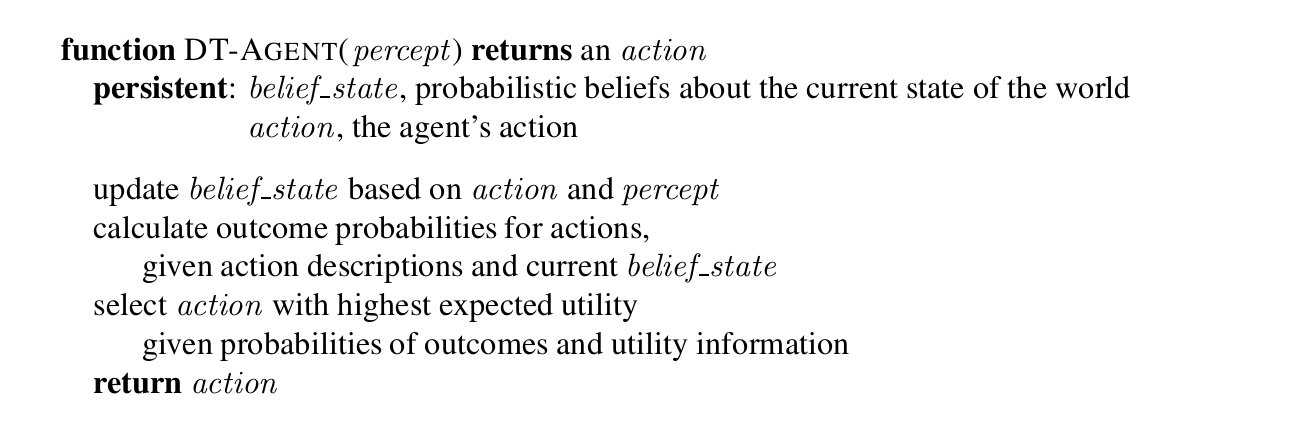
\includegraphics[width=1\linewidth]{algorithms/DT Agent.png}
    \label{fig:DT_agent_algorithm}
\end{figure}

\subsection{Probability Theory}
For the agent to represent and use probabilistic information, we need a formal language called \textbf{probability theory}.

In probability theory, the set of all possible worlds is called the \textbf{sample space}. The possible worlds are \underline{mutually exclusive} and \underline{exhaustive}. The sample space is represented by the Greek letter $\Omega$ and the elements of the space are referred with the letter $\omega$. A fully specified probability model associates a numerical probability $P(\omega)$ with each possible world. The basic axioms of probability theory says that every possible world has a probability between 0 and 1 and the total probability of the set of possible worlds is 1:
$$\forall\omega \;\; 0\le P(\omega) \le 1 \;\; and \;\; \sum_{\omega\in\Omega}P(\omega) = 1$$

Probabilistic assertions and queries are not usually about particular possible worlds, but about some sets of them: in particular, these sets are called \textbf{events}. A set of worlds corresponds to a proposition in a formal language. The probability associated with a proposition is defined to be the sum of all the probabilities of the worlds in which it holds
$$\forall \; proposition \; \phi, \;\; P(\phi)=\sum_{\omega\in\phi}P(\omega)$$

We define \textbf{unconditional probability} as the degree of belief in a proposition in the absence of any other evidence. On the other hand, we define \textbf{conditional probability} as the degree of belief in a proposition given some evidence that has already been revealed. We write $P(a|b)$, pronounced "the probability of $a$ given $b$", and it is mathematically defined in terms of unconditional probabilities as follows:
$$P(a|b) = \frac{P(a\land b)}{P(b)}$$
which holds whenever $P(b)>0$. This equation can be rearranged in a different form, called the \textbf{product rule}:
\begin{align*}
    P(a\land b) &= P(a|b)P(b)\\
    P(a\land b) &= P(b|a)P(a)
\end{align*}

\subsubsection{Variables and Probability Distributions}
Variables in probability theory are called \textbf{random variables} and their names begin with an uppercase letter. Every random variable is a function that maps from the domain of possible worlds $\Omega$ to the set of values it can take on. Name for values are always lowercase, so we can write $\sum_xP(X=x)$ to sum over the values of $X$. By convention, propositions of the form $A=true$ are abbreviated with $a$, while $A=false$ is abbreviated with $\neg a$. Variables can have infinite ranges, either discrete or continuous. We can also combine elementary propositions using the connectives of propositional logic, keeping in mind that it is common to use commas for conjunction.

Sometimes it is necessary to talk about the probabilities of all the possible values of a random variable. We can write
\begin{align*}
    P(X=x_1) &= y_1 \\
    P(X=x_2) &= y_2 \\
    &\;\;\vdots     \\
    P(X=x_n) &= y_n 
\end{align*}
abbreviated with the following notation
$$\textbf{P}(x) = \langle y_1, y_2, ..., y_n\rangle$$
where the bold $\textbf{P}$ indicates that the result is a vector of numbers, assuming a predefined ordering. The $\textbf{P}(X)$ statement defines a \textbf{probability distribution} for the random variable $X$, that is an assignment of a probability for each possible value for $X$. The $\textbf{P}$ notation can also be used for conditional distributions: $\textbf{P}(X|Y)$ gives the values of $P(X=x_i|Y=y_j)$ for each possible $i, j$ pair.

For continuous variables, it is not possible to write out the entire distribution as a vector,because there are infinitely many values. Instead we can define a so called \textbf{probability density function} (\textbf{pdfs} for short), which defines the probability that a random variable $X$ takes on some value $x$. We write the probability density fora continuous random variable $X$ at value $x$ as $P(X=x)$, or $P(x)$ for short. The intuitive definition of $P(x)$ is the following:
$$P(x) = \lim_{dx\to0}P(x\le X\le x+dx)/dx$$

In addition to distributions on single variables, we can use commas to denote the distribution on multiple variables. The resulting tables of probabilities are called \textbf{joint probability distribution}. A probability model is completely determined by the joint distribution for all of the random variables, which gives us the \textbf{full joint probability distribution}, which in principle is sufficient for calculating the probabilities of any proposition.

\subsubsection{Probability Axioms}
The basic axioms of probability imply certain relationships among the degrees of belief that can be accorded to logically related propositions. One important example is the relationship between the probability of a proposition and the probability of its negation
\begin{align*}
    P(\neg a) &= \sum_{\omega\in \neg a}P(\omega)\\
    &= \sum_{\omega\in \neg a}P(\omega) + \sum_{\omega\in a}P(\omega) - \sum_{\omega\in a}P(\omega)\\
    &= \sum_{\omega\in\Omega}P(\omega) - \sum_{\omega\in a}P(\omega) \\
    &= 1 - P(a)
\end{align*}
We can also derive the well-known formula for the probability of a disjunction, also called the \textbf{inclusion-exclusion principle}:
$$P(a \lor b) = P(a)+P(b)-P(a\land b)$$

\subsubsection{Probabilistic Inference}
Probabilistic inference is the computation of posterior probabilities for query propositions given some observed evidence. We can use the full joint distribution table as the "knowledge base" from which we can derive the answers to all questions.

One particular common task is to extract the distribution over some subset of variables or a single variable. We can obtains such value by summing up the probabilities for each possible value of the other variable (adding together rows or columns), obtaining the so called \textbf{marginal probability}.The process of extracting the marginal probability from the table is called \textbf{marginalization}. The general marginalization rule for any set of variables $\textbf{Y}$ and $\textbf{Z}$ is 
$$\textbf{P}(\textbf{Y})=\sum_\textbf{z}\textbf{P}(\textbf{Y},\textbf{Z}=\textbf{z})$$
where $\sum_\textbf{z}$ sums over all the possible combinations of values of the set of variables $\textbf{Z}$. In other words
$$P(a) = P(a\land b) + P(a\land \neg b)$$

Using the product rule, we can replace $\textbf{P}(\textbf{Y}, \textbf{z})$ with $\textbf{P}(\textbf{Y}|\textbf{z})P(\textbf{z})$, obtaining the \textbf{conditioning rule}
$$\textbf{P}(\textbf{Y}) = \sum_\textbf{z}\textbf{P}(\textbf{Y}|\textbf{z})P(\textbf{z})$$
or, in other words
$$P(a) = P(a|b)P(b)+P(a|\neg b)P(\neg b)$$

In most cases, we are interested in computing conditional probabilities od some variables, given evidence about some others. Conditional probabilities can be  first calculated with the equation $P(a|b) = P(a\land b) / P(b)$
to obtain an expression in terms of unconditional probabilities and then evaluating the expression from the full joint distribution. The term $P(b)$ in the expression for conditional probabilities can be seen as a normalization constant for the distribution $\textbf{P}(A|b)$, ensuring that it adds up to 1. We denote such constant with $\alpha$, so the expression can be written as
$$\textbf{P}(A|b)=\alpha \textbf{P}(A\land b)$$
This notation is quite useful in practice because we often don't know the value of \textbf{P(b)}, but we can temporarily ignore it and later infer it by knowing that probabilities must add up to 1.

We can generalize the inference procedure. Let $\textbf{E}$ be the list of evidence variables and $\textbf{e}$ the list of observed values for them, and let $\textbf{Y}$ be the remaining unobserved variables (those that are not necessary to calculate the required probability). The query is $\textbf{P}(X|\textbf{e})$ and can be evaluated as follows
$$\textbf{P}(X|\textbf{e})=\alpha\textbf{P}(X,\textbf{e})=\alpha\sum_\textbf{y}\textbf{P}(X,\textbf{e},\textbf{y})$$
where the summation is over all possible combinations of values of the unobserved variables $\textbf{Y}$. Notice that together the variables $X$, $\textbf{E}$ and $\textbf{Y}$ constitute the complete set of variables for the domain, so $\textbf{P}(X,\textbf{e},\textbf{y})$ represents a subset of probabilities from the full joint distribution.

Given the full joint distribution, the previous equation can answer any probabilistic query for discrete variables in that domain. However, this strategy does not scale up very well: in a discrete domain, given $n$ boolean variables, it requires an input table of size $O(2^n)$ and takes $O(2^n)$ time to process the table.

\subsubsection{Independence}
Independence is the knowledge that the occurrence of one event does not affect the probability of one other event. Mathematically, can be written as
\begin{align*}
    \begin{array}{ccccc}
        \textbf{P}(X|Y) = \textbf{P}(X) & & \textbf{P}(Y|X) = \textbf{P}(Y) & &\textbf{P}(X, Y) = \textbf{P}(X)\textbf{P}(Y)
    \end{array}
\end{align*}
or, in other words
\begin{align*}
    \begin{array}{ccccc}
        P(a|b) = P(a) & & P(b|a) = P(b) & & P(a \land b) = P(a)P(b)
    \end{array}
\end{align*}

Independence assertions are usually based on the knowledge of the domain. If the complete set of variables can be divided into independent subsets, then the full joint distribution can be factored into separate joint distributions on those subsets. When they are available, independence assertions can help in reducing the size of the domain representation and the complexity of the inference problem.

\subsubsection{Bayes' Rule}
We have previously defined the \textbf{product rule}, mathematically written as
\begin{align*}
    \begin{array}{ccc}
        P(a\land b) = P(a|b)P(b) & or & P(a\land b) = P(b|a)P(a)
    \end{array}
\end{align*}
By equating the two right-handed sides of the equations, we obtain that
$$P(b|a) = \frac{P(a|b)P(b)}{P(a)}$$
also known as the \textbf{Bayes' theorem}, which underlies most of modern AI systems for probabilistic inference. More generally we can write the Bayes' rule as follows
$$\textbf{P}(Y|X) = \frac{\textbf{P}(X|Y)\textbf{P}(Y)}{\textbf{P}(X)}$$

\subsection{Bayesian Networks}
As already said, full joint probability distribution can answer any question about a domain, but can become too large as the number of variables grows. Independence and conditional independence can drastically reduce the number of probabilities required to define the full joint distribution. A \textbf{Bayesian network} is a data structure used to represent the dependencies among variables and can represent any full joint probability distribution in a concise manner. 

A Bayesian network is a \textbf{directed acyclic graph} in which each node is annotated with quantitative probability information, as follows:
\begin{enumerate}
    \item Each node correspond to a random variable, which may be discrete or continuous.
    \item Directed arrows connect pairs of nodes. If there is an arrow from node $X$ to node $Y$, $X$ is said to be the parent of $Y$. The graph has no directed cycles and hence is a directed acyclic graph (DAG for short).
    \item Each node $X_i$ has associated probability information $\theta(X_i|Parents(X_i))$ that quantifies the effect of the parents on the node using a finite number of parameters. 
\end{enumerate}

The topology of the network specifies the conditional independence relationships that hold in the domain: the intuitive meaning of an arrow is that $X$ has a direct influence on $Y$, which suggests that causes should be parents of effects. Once the topology is laid out, we need only to specify the local probability information for each variable in the form of a conditional distribution given its parents. The full joint distribution for all the variables is defined by the topology and the local probability information, which is represented by a \textbf{conditional probability table} (CPT for short). Each row of the CPT contains the conditional probability of each node value for a \textbf{conditioning case}, which is a possible combination of values for the parent nodes. Each row \underline{must} sum to 1. A node with no parents has only one row, representing the prior probabilities of each possible value of the variable.

Assuming that the Bayesian network contains $n$ variables $X_1, ..., X_n$, a generic entry in the joint distribution is denoted with $P(X_1=x_1\land...\land X_n=x_n)$, or $P(x_1,...,x_n)$ for short. Bayesian nets defines each entry in the joint distribution as follows:
$$P(x_1,...,x_n) = \prod_{i=1}^{n}\theta(x_1\;|\;parents(X_i))$$
where $parents(X_i)$ denotes the values of $Parents(X_i)$ that appear in $x_1, ..., x_n$. Thus, each entry in the joint distribution is represented by the product of the appropriate elements of the local conditional distribution in the Bayesian net. The Bayesian network is a representation of the joint probability distribution, so it can be used to answer any query by summing up all the relevant joint probability values, each calculated by multiplying probabilities from the local conditional distributions. 

Now, the $\theta(x_i|parents(X_i))$ parameters in the previous equation can be proved to be exactly the conditional probabilities $P(x_i|parents(X_i))$ implied by the jointed distribution. The conditional probabilities can be computed as follows:
\begin{align*}
    P(x_i|parents(X_i)) &= \frac{P(x_i, parents(X_i))}{P(parents(X_i))}\\
                        &= \frac{\sum_\textbf{y}P(x_i, parents(X_i),\textbf{y})}{\sum x_i',\textbf{y} P(x_i', parents(x_i), \textbf{y}}
\end{align*}
\clearpage
Where $\textbf{y}$ represents the values of all variables other than $X_i$ and its parents. So, from the last line of the equation we can prove that $P(x_i|parents(X_i)) = \theta(x_i|parents(X_i))$, hence we can write that
$$P(x_1,...,x_n) = \prod_{i=1}^nP(x_i|parents(X_i))$$

This means that when we estimate the values for the local conditional distribution, they must be the actual conditional probabilities for the variable given its parents. 

In order to construct a Bayesian network, we first need to rewrite the entries in the joint distribution in terms of conditional probabilities, using the \textbf{chain rule}:
\begin{align*}
P(x_1,...,x_n) &= P(x_n|x_{n-1},...,x_1)P(x_{n-1}|x_{n-2},...,x_1)\cdots P(x_2|x_1)P(x_1) \\
               &= \prod_{i=1}^nP(x_i|x_{i-1},...,x_1)
\end{align*}
We can see that the specification of the joint distribution is equivalent to the general assertion that, for every variable in the network,
$$\textbf{P}(X_i|X_{i-1},...,X_1)= \textbf{P}(X_i|Parents(X_i))$$
provided that $Parents(X_i) \subseteq \{X_{i-1},...,X_1\}$. This condition is satisfied by numbering the node in \textbf{topological order}.

\subsubsection{Exact Inference}
The basic task for any probabilistic inference system is to compute the posterior probability distribution for a set of query variables, given some observed \textbf{event}. As seen before, we use the following notation:
\begin{itemize}
    \item $X$ denotes the query variable.
    \item $\textbf{E}$ denotes the set of evidence variables $E_1, ..., E_n$.
    \item $\textbf{e}$ denotes a particular observed event.
    \item $\textbf{Y}$ denotes the hidden variables\footnote{\textbf{Hidden variables} are the nodes in the Bayesian networks which are neither input nor output, but are essential to structure the network. These nodes are non-evidence and non-query variables.}.
    \item $\alpha$ denotes the normalization factor. 
\end{itemize}
So the complete set of variables is $\{X\}\cup\textbf{E}\cup\textbf{Y}$, and a typical query asks the posterior probability distribution $\textbf{P}(X|\textbf{e})$.

As already said, any conditional probability can be computed by summing terms from the full joint distribution: specifically, a query $\textbf{P}(X|\textbf{e})$ can be answered using the equation 
$$\textbf{P}(X|\textbf{e})=\alpha\textbf{P}(X,\textbf{e})=\alpha\sum_\textbf{y}\textbf{P}(X,\textbf{e},\textbf{y})$$

Therefore, a query can be answered using a Bayesian network by computing sums of products of conditional probabilities from the network.

There are several structures that can arise in Bayesian networks, which determine the influences some variables can have on others:
\begin{itemize}
    \item $X \rightarrow Y$: $X$ influences $Y$ (causal).
    \item $X \leftarrow Y$: $X$ influences $Y$ (evidential).
    \item $X \rightarrow W \rightarrow Y$: $X$ influences $Y$ (causal chain).
    \item $X \leftarrow W \leftarrow Y$: $X$ influences $Y$ (evidential).
    \item $X \leftarrow W \rightarrow Y$: $X$ influences $Y$.
    \item $X \rightarrow W \leftarrow Y$ (V-structure): $X$ does \underline{not} influence $Y$.
\end{itemize}

\noindent
In Bayesian networks, active trails describe a path along which information or dependencies can flow between nodes in the network. This concept is crucial for understanding the conditional independence relationships in the network. It can be demonstrated that a trail $X_1-...-X_n$ is active if it has no V-structures. Active trails can help in efficient inference by identifying which variables influence others directly or indirectly in the presence of observed evidence.

The situation becomes more complex when evidence is added to the equation. For the cases in which the trail is in the form of $X \rightarrow Y$ and $X \leftarrow Y$, there are differences, since the evidence about some variable $Z$ plays no role in how $X$ and $Y$ effect each other. For the other cases:
\begin{itemize}
    \item $X \rightarrow W \rightarrow Y$: $X$ influences $Y$ only if $W\notin Z$; in other cases $X$ does not influence $Y$.
    \item $X \leftarrow W \leftarrow Y$: $X$ influences $Y$ only if $W\notin Z$; in other cases $X$ does not influence $Y$.
    \item $X \leftarrow W \rightarrow Y$: $X$ influences $Y$ only if $W\notin Z$; in other cases $X$ does not influence $Y$.
    \item $X \rightarrow W \leftarrow Y$ (V-structure): $X$ cannot influence $Y$ if $W$ and \textit{\underline{all} its descendant} are not in $Z$; in other cases, $X$ can influence $Y$ if $W$ or one of its descendant are in $Z$.
\end{itemize}

\noindent
In general, a trail $X_1-...-X_n$ is active given evidence $Z$ if for any V-structure $X_{i-1}\rightarrow X_i \leftarrow X_{i+1}$, $X_i$ or one of its descendant is in $Z$. No other $X_i$ in V-structures is in $Z$.

\subsubsection{Approximate Inference}
Approximate inference in Bayesian networks refers to methods used to estimate posterior probabilities when exact inference is computationally infeasible. This is common in large networks with many variables, where exact methods (like variable elimination or junction trees) become intractable due to exponential growth in computational complexity.

The most used strategy in approximate inference is \textbf{sampling}, which relies on iteratively generating samples from the distribution to estimate posterior probabilities. This allows to do inference without enumerating all the possible configurations, as done in exact inference.

A general method is \textbf{rejection sampling}, which first generates samples from the prior distribution specified by the network, then it rejects all those that do not match the evidence and finally, the estimate $\hat{P}(X=x|\textbf{e})$ is obtained by counting all occurrences of $X=x$ in the remaining samples. 

More formally, let $\hat{\textbf{P}}(X|\textbf{e})$ be the estimated distribution that the algorithm returns. This distribution is computed by normalizing $\textbf{N}_{PS}(X,\textbf{e})$, which is the vector of sample counts for each value of $X$ where the sample agrees with the evidence $\textbf{e}$:

$$\hat{\textbf{P}}(X|\textbf{e})=\alpha\textbf{N}_{PS}(X,\textbf{e})=\frac{\textbf{N}_{PS}(X|\textbf{e})}{N_{PS}(\textbf{e})}$$

which gives

$$\hat{\textbf{P}}(X|\textbf{e})\approx\frac{\textbf{P}(X, \textbf{e})}{P(\textbf{e})}=\textbf{P}(X|\textbf{e})$$

That is, rejection sampling produces a consistent estimate of the true probability. rejection sampling can be quite inefficient since it might need to generate a huge number of samples, in order to do inference from the model.

\clearpage
\appendix
\section{Logic}\label{appendix:Logic}
De Morgan rules:
\begin{align*}
    \alpha \land \beta &\equiv \beta \land \alpha \\
    \alpha \lor \beta &\equiv \beta \lor \alpha \\
    (\alpha \land \beta)\land \gamma &\equiv \alpha \land (\beta \land \gamma) \\
    (\alpha \lor \beta)\lor \gamma &\equiv \alpha \lor (\beta \lor \gamma) \\
    \neg (\neg \alpha) &\equiv \alpha \\
    \alpha \Rightarrow \beta &\equiv \neg \beta \Rightarrow \neg \alpha \\
    \alpha \Rightarrow \beta &\equiv \neg \alpha \lor \beta \\
    \alpha\Leftrightarrow\beta &\equiv (\alpha\Rightarrow\beta) \land (\beta\Rightarrow\alpha) \\
    \neg (\alpha \land \beta) &\equiv (\neg \alpha \lor \neg \beta) \\
    \neg (\alpha \lor \beta) &\equiv (\neg \alpha \land \neg \beta) \\
    \alpha \land (\beta \lor \gamma) &\equiv (\alpha\land\beta)\lor(\alpha\land\gamma) \\
    \alpha \lor (\beta \land \gamma) &\equiv (\alpha \lor \beta)\land(\alpha \lor \gamma)
\end{align*}

\end{document}
    